\documentclass[aspectratio=169, 10pt]{beamer}

% --- GÓI HỌC THUẬT & FONT TIẾNG VIỆT CHO XELATEX ---
\usepackage{fontspec}
\setmainfont{Arial}
\setsansfont{Arial}
\setmonofont{Consolas}

\usepackage{amsmath,amssymb}
\usepackage{graphicx}
\usepackage{booktabs}
\usepackage{tabularx}
\usepackage{multicol}
\usepackage{listings}
\usepackage{xcolor}
\usepackage{tikz}
\usetikzlibrary{shapes,arrows,positioning,fit,backgrounds,calc}
\usepackage{tcolorbox}
\tcbuselibrary{skins,breakable,listings}

% --- ĐỊNH NGHĨA MÀU SẮC CHUẨN ĐẠI HỌC & C# .NET ---
\definecolor{UniNavy}{RGB}{15, 44, 89}        % Xanh hải quân chủ đạo (#0F2C59)
\definecolor{UniBlue}{RGB}{29, 93, 155}       % Xanh Slate (#1D5D9B)
\definecolor{CSharpPurple}{RGB}{104, 33, 122} % Tím nhận diện C# & Visual Studio (#68217A)
\definecolor{UniLightBlue}{RGB}{232, 241, 252}% Nền xanh nhạt
\definecolor{UniOrange}{RGB}{225, 112, 18}    % Cam nhấn mạnh (#E17012)
\definecolor{UniGreen}{RGB}{30, 132, 73}      % Xanh lá thực hành (#1E8449)
\definecolor{UniDark}{RGB}{33, 37, 41}        % Màu chữ chính / nền console
\definecolor{CodeBg}{RGB}{248, 249, 250}      % Nền code
\definecolor{CSharpKeyword}{RGB}{0, 0, 255}   % Xanh dương từ khóa C#
\definecolor{CSharpString}{RGB}{163, 21, 21}  % Đỏ chuỗi C#
\definecolor{CSharpComment}{RGB}{0, 128, 0}   % Xanh lá chú thích C#

% --- CẤU HÌNH THEME BEAMER MADRID WIDESCREEN ---
\usetheme{Madrid}
\usecolortheme{whale}

\setbeamercolor{palette primary}{bg=UniNavy, fg=white}
\setbeamercolor{palette secondary}{bg=CSharpPurple, fg=white}
\setbeamercolor{palette tertiary}{bg=UniNavy!85, fg=white}
\setbeamercolor{palette quaternary}{bg=UniNavy, fg=white}

\setbeamercolor{structure}{fg=UniNavy}
\setbeamercolor{titlelike}{parent=structure, fg=UniNavy}
\setbeamercolor{frametitle}{bg=UniNavy, fg=white}
\setbeamercolor{frametitle continuation}{fg=white}
\setbeamercolor{normal text}{fg=UniDark}

% Cấu hình khối thông tin (Blocks)
\setbeamercolor{block title}{bg=UniBlue, fg=white}
\setbeamercolor{block body}{bg=UniLightBlue!40, fg=UniDark}
\setbeamercolor{block title example}{bg=UniGreen, fg=white}
\setbeamercolor{block body example}{bg=UniGreen!10, fg=UniDark}
\setbeamercolor{block title alerted}{bg=UniOrange, fg=white}
\setbeamercolor{block body alerted}{bg=UniOrange!10, fg=UniDark}

% Cấu hình Footline chuyên nghiệp
\setbeamertemplate{navigation symbols}{}
\setbeamertemplate{footline}{
  \leavevmode%
  \hbox{%
    \begin{beamercolorbox}[wd=.35\paperwidth,ht=2.5ex,dp=1.1ex,left,leftskip=2ex]{author in head/foot}%
      \usebeamerfont{author in head/foot}\textbf{Lớp IT26M} | Lập trình C\# \& .NET
    \end{beamercolorbox}%
    \begin{beamercolorbox}[wd=.45\paperwidth,ht=2.5ex,dp=1.1ex,center]{title in head/foot}%
      \usebeamerfont{title in head/foot}Chương 3: Lập trình Ứng dụng C\# Căn bản
    \end{beamercolorbox}%
    \begin{beamercolorbox}[wd=.20\paperwidth,ht=2.5ex,dp=1.1ex,right,rightskip=2ex]{date in head/foot}%
      \usebeamerfont{date in head/foot}\insertframenumber{} / \inserttotalframenumber
    \end{beamercolorbox}%
  }%
  \vskip0pt%
}

% --- CẤU HÌNH GÓI LISTINGS CHO C# & TERMINAL ---
\lstdefinelanguage{CSharpCustom}{
  keywords={abstract, as, base, bool, break, byte, case, catch, char, checked, class, const, continue, decimal, default, delegate, do, double, else, enum, event, explicit, extern, false, finally, fixed, float, for, foreach, goto, if, implicit, in, int, interface, internal, is, lock, long, namespace, new, null, object, operator, out, override, params, private, protected, public, readonly, ref, return, sbyte, sealed, short, sizeof, stackalloc, static, string, struct, switch, this, throw, true, try, typeof, uint, ulong, unchecked, unsafe, ushort, using, virtual, void, volatile, while, async, await, var},
  keywordstyle=\color{CSharpKeyword}\bfseries,
  ndkeywords={Console, String, Math, Convert, int, double, float, char, bool},
  ndkeywordstyle=\color{CSharpPurple}\bfseries,
  sensitive=true,
  comment=[l]{//},
  morecomment=[s]{/*}{*/},
  commentstyle=\color{CSharpComment}\itshape,
  stringstyle=\color{CSharpString},
  morestring=[b]",
  morestring=[b]'
}

\lstset{
  language=CSharpCustom,
  basicstyle=\ttfamily\scriptsize,
  numbers=left,
  numberstyle=\tiny\color{gray},
  stepnumber=1,
  numbersep=6pt,
  backgroundcolor=\color{CodeBg},
  frame=single,
  rulecolor=\color{black!20},
  tabsize=4,
  showstringspaces=false,
  breaklines=true,
  breakatwhitespace=true,
  columns=flexible,
  keepspaces=true,
  xleftmargin=12pt,
  framexleftmargin=10pt
}

% Style cho console output
\lstdefinestyle{terminalStyle}{
  basicstyle=\ttfamily\scriptsize\color{white},
  backgroundcolor=\color{UniDark},
  frame=single,
  rulecolor=\color{UniNavy},
  numbers=none,
  xleftmargin=6pt,
  framexleftmargin=6pt
}

% --- THÔNG TIN TRANG TIÊU ĐỀ ---
\title[\textbf{Lập trình C\# \& .NET -- Chương 3}]{\textbf{\LARGE KỸ THUẬT LẬP TRÌNH C\#}}
\subtitle{\textbf{\large Chương 3: Giới thiệu Lập trình Ứng dụng C\# (Introduction to C\# App Programming)}}
\author[\textbf{Khoa CNTT -- IT26M}]{\textbf{BÀI GIẢNG CHUẨN ĐẠI HỌC (3 TIẾT TÍCH HỢP)}\\Giáo trình: \textit{Visual C\# How to Program} (Deitel \& Deitel)}
\institute[\textbf{Lớp IT26M}]{\textbf{Khoa Công nghệ Thông tin -- Đại học Đông Á}\\\textbf{Đối tượng:} Lớp IT26M (Khóa 2026)}
\date[\textbf{2026}]{\textbf{Học kỳ I -- Năm học 2026}}

\begin{document}

% ==============================================================================
% SLIDE 1: TRANG TIÊU ĐỀ BÀI GIẢNG
% ==============================================================================
\begin{frame}[plain]
  \titlepage
  \begin{center}
    \scriptsize \color{gray} Bản quyền bài giảng thuộc Bộ môn Kỹ thuật Lập trình -- Phục vụ đào tạo Đại học chính quy
  \end{center}
\end{frame}

% ==============================================================================
% SLIDE 2: MỤC TIÊU BÀI HỌC & CHUẨN ĐẦU RA (CLOs)
% ==============================================================================
\begin{frame}{Mục tiêu Bài học \& Chuẩn đầu ra (CLOs)}
  \begin{block}{\textbf{Chuẩn đầu ra sinh viên cần đạt được sau buổi học 3 tiết:}}
    \begin{itemize}
      \item \textbf{CLO 3.1 (Understand):} Giải thích kiến trúc ứng dụng Console C\#, vai trò của phương thức \texttt{static void Main()}, chỉ thị \texttt{using System;}, khối lệnh \texttt{\{\}} và quy ước PascalCase.
      \item \textbf{CLO 3.2 (Apply):} Vận dụng thành thạo xuất dữ liệu (\texttt{Console.Write}, \texttt{Console.WriteLine}), ký tự thoát (\texttt{\textbackslash n}, \texttt{\textbackslash t}, \texttt{\textbackslash\textbackslash}, \texttt{\textbackslash"}) và Nội suy chuỗi C\# 6 (\texttt{\$"...\{var\}..."}).
      \item \textbf{CLO 3.3 (Apply):} Khai báo biến \texttt{int}, nhập dữ liệu bằng \texttt{Console.ReadLine()}, ép kiểu \texttt{int.Parse()} và hiểu rõ cơ chế ô nhớ RAM (đọc không phá hủy vs ghi đè phá hủy).
      \item \textbf{CLO 3.4 (Apply):} Sử dụng các toán tử số học (\texttt{+}, \texttt{-}, \texttt{*}, \texttt{/}, \texttt{\%}), nắm vững thứ tự ưu tiên (precedence) và chuyển đổi công thức đại số sang mã C\#.
      \item \textbf{CLO 3.5 (Create):} Xây dựng cấu trúc rẽ nhánh ra quyết định với câu lệnh \texttt{if}, kết hợp toán tử quan hệ (\texttt{<}, \texttt{<=}, \texttt{>}, \texttt{>=}) và bình đẳng (\texttt{==}, \texttt{!=}).
    \end{itemize}
  \end{block}
  \vspace{-2mm}
  \begin{exampleblock}{\textbf{Phương pháp sư phạm:}}
    Học qua ví dụ thực chiến (Case-Based Learning): Từ \textbf{Welcome1} $\to$ \textbf{Welcome4} $\to$ \textbf{Addition} $\to$ \textbf{Comparison}.
  \end{exampleblock}
\end{frame}

% ==============================================================================
% SLIDE 3: TIẾN TRÌNH BÀI HỌC 3 TIẾT
% ==============================================================================
\begin{frame}{Tiến trình Bài học 3 Tiết (150 Phút Tích hợp)}
  \begin{columns}[T]
    \begin{column}{0.32\textwidth}
      \begin{tcolorbox}[colback=UniNavy!5,colframe=UniNavy,title=\textbf{TIẾT 1 (50')},fonttitle=\small\bfseries]
        \textbf{Cấu trúc Console App}
        \begin{itemize}\scriptsize
          \item Kiến trúc Console vs GUI
          \item Phân tích \texttt{Welcome1.cs}
          \item Chú thích \& \texttt{using System;}
          \item Lớp \& Phương thức \texttt{Main()}
          \item \texttt{Console.WriteLine()}
          \item Tạo Console App trong VS
          \item IntelliSense \& Parameter Info
          \item Xử lý lỗi Error List
          \item \textbf{[LAB 1]:} Code Welcome1, 2
        \end{itemize}
      \end{tcolorbox}
    \end{column}

    \begin{column}{0.32\textwidth}
      \begin{tcolorbox}[colback=CSharpPurple!5,colframe=CSharpPurple,title=\textbf{TIẾT 2 (50')},fonttitle=\small\bfseries]
        \textbf{Biến, Bộ nhớ \& Số học}
        \begin{itemize}\scriptsize
          \item Escape Sequences (\texttt{Welcome3})
          \item Nội suy chuỗi (\texttt{Welcome4})
          \item Khai báo biến \& Kiểu \texttt{int}
          \item \texttt{Console.ReadLine()} \& \texttt{Parse}
          \item Toán tử gán (\texttt{=})
          \item Ô nhớ: Non- vs Destructive
          \item 5 Toán tử số học (+, -, *, /, \%)
          \item Chia nguyên \& Chia dư (\%)
          \item Thứ tự ưu tiên \& Đa thức
          \item \textbf{[LAB 2]:} Ứng dụng Addition
        \end{itemize}
      \end{tcolorbox}
    \end{column}

    \begin{column}{0.32\textwidth}
      \begin{tcolorbox}[colback=UniGreen!5,colframe=UniGreen,title=\textbf{TIẾT 3 (50')},fonttitle=\small\bfseries]
        \textbf{Rẽ nhánh \& Thực hành}
        \begin{itemize}\scriptsize
          \item Câu lệnh điều kiện đơn \texttt{if}
          \item Toán tử so sánh (==, !=, <, >)
          \item Phân biệt sống còn \texttt{=} vs \texttt{==}
          \item Case Study \texttt{Comparison.cs}
          \item Cạm bẫy dấu \texttt{;} sau \texttt{if}
          \item Khối lệnh \texttt{\{\}} compound
          \item Bảng tổng kết toán tử
          \item Quy chuẩn Clean Code
          \item \textbf{[LAB 3]:} Đồ án Comparison
          \item Giới thiệu Đồ án lớn
        \end{itemize}
      \end{tcolorbox}
    \end{column}
  \end{columns}
\end{frame}

% ==============================================================================
% SLIDE 4: CONSOLE APP VS GUI
% ==============================================================================
\begin{frame}{Khái niệm: Ứng dụng Console (CLI) vs Ứng dụng Đồ họa (GUI)}
  \begin{columns}[T]
    \begin{column}{0.48\textwidth}
      \begin{block}{\textbf{Ứng dụng Console (Command-Line)}}
        \begin{itemize}\small
          \item Giao tiếp qua văn bản thuần túy (Text-based): xuất ra màn hình Command Prompt / Terminal và nhận nhập liệu từ bàn phím.
          \item Không cần xử lý các sự kiện đồ họa phức tạp (chuột, kéo thả, vẽ lại cửa sổ).
          \item \textbf{Mục đích học tập:} Tập trung 100\% vào \textbf{tư duy thuật toán, cấu trúc điều khiển, kiểu dữ liệu và luồng thực thi logic} của C\#.
          \item Dùng phổ biến trong: Dịch vụ nền tảng (Microservices), Script tự động hóa, Điện toán đám mây.
        \end{itemize}
      \end{block}
    \end{column}

    \begin{column}{0.48\textwidth}
      \begin{exampleblock}{\textbf{Mối liên hệ với Chương 2 (Windows Forms)}}
        \begin{itemize}\small
          \item Ở Chương 2, chúng ta đã dùng chuột kéo thả để tạo giao diện GUI trực quan (\texttt{Form}, \texttt{Button}, \texttt{Label}).
          \item \textbf{Bản chất:} Phía sau mỗi sự kiện nhấp nút (Click Event) đều cần những dòng lệnh logic C\# thuần túy để tính toán!
          \item Chương 3 trang bị cho các em nền tảng lập trình mã nguồn nòng cốt để viết logic bên trong các hàm sự kiện đó.
        \end{itemize}
      \end{exampleblock}
    \end{column}
  \end{columns}
  \vspace{2mm}
  \begin{alertblock}{\textbf{Thông điệp cốt lõi:}}
    Một kỹ sư phần mềm giỏi phải nắm chắc cách viết code dòng lệnh trước khi xây dựng các hệ thống đồ họa hay web quy mô lớn!
  \end{alertblock}
\end{frame}

% ==============================================================================
% SLIDE 5: TIẾT 1 DIVIDER
% ==============================================================================
\begin{frame}[plain]
  \vfill
  \centering
  \begin{beamercolorbox}[sep=8pt,center,shadow=true,rounded=true]{palette primary}
    {\Huge \textbf{TIẾT 1}}\\[2mm]
    {\Large \textbf{CẤU TRÚC CONSOLE APP, WELCOME1 ĐẾN WELCOME4, INTELLISENSE \& ERROR LIST}}
  \end{beamercolorbox}
  \vfill
\end{frame}

% ==============================================================================
% SLIDE 6: CODE STUDY 1: WELCOME1.CS
% ==============================================================================
\begin{frame}[fragile]{Chương trình C\# Đầu tiên: \texttt{Welcome1.cs}}
  \begin{columns}[T]
    \begin{column}{0.55\textwidth}
      \begin{tcolorbox}[colback=CodeBg,colframe=UniNavy,title=\textbf{Welcome1.cs (Fig. 3.1)},fonttitle=\small\bfseries]
\begin{lstlisting}
// Fig. 3.1: Welcome1.cs
// Text-displaying app.
using System;

class Welcome1
{
   // Main method begins execution of C# app
   static void Main()
   {
      Console.WriteLine("Welcome to C# Programming!");
   } // end Main
} // end class Welcome1
\end{lstlisting}
      \end{tcolorbox}
    \end{column}

    \begin{column}{0.43\textwidth}
      \begin{exampleblock}{\textbf{Cấu trúc 4 Khối Nòng cốt}}
        \begin{enumerate}\small
          \item \textbf{Dòng 1--2:} Chú thích tài liệu hóa (\texttt{// Comment}).
          \item \textbf{Dòng 3:} Chỉ thị nhập không gian tên (\texttt{using System;}).
          \item \textbf{Dòng 5--12:} Khai báo lớp đối tượng (\texttt{class Welcome1}).
          \item \textbf{Dòng 8--11:} Phương thức thực thi chính (\texttt{static void Main()}).
        \end{enumerate}
      \end{exampleblock}

      \begin{tcolorbox}[colback=UniDark,colframe=black,title=\textbf{Màn hình Console Output},fonttitle=\scriptsize\bfseries]
        \color{white}\ttfamily\scriptsize
        Welcome to C\# Programming!
      \end{tcolorbox}
    \end{column}
  \end{columns}
\end{frame}

% ==============================================================================
% SLIDE 7: CHÚ THÍCH & CHỈ THỊ USING
% ==============================================================================
\begin{frame}{Cú pháp Căn bản: Chú thích (Comments) \& Chỉ thị \texttt{using}}
  \begin{columns}[T]
    \begin{column}{0.48\textwidth}
      \begin{block}{\textbf{1. Chú thích trong C\# (Comments)}}
        \begin{itemize}\small
          \item \textbf{Chú thích một dòng (\texttt{//}):} Trình biên dịch C\# bỏ qua tất cả ký tự từ \texttt{//} đến hết dòng.
          \item \textbf{Chú thích nhiều dòng (\texttt{/* ... */}):} Dùng để chú thích một khối văn bản dài hoặc tạm thời vô hiệu hóa đoạn mã.
          \item \textbf{Vai trò kỹ sư:} Tăng tính rõ ràng, dễ bảo trì cho mã nguồn. Không làm tăng kích thước tệp \texttt{.exe} được biên dịch.
        \end{itemize}
      \end{block}
      \begin{exampleblock}{\textbf{Ví dụ:}}
        \texttt{// Day la chu thich 1 dong}\\
        \texttt{/* Chu thich\\
        \hspace*{4mm}nhieu dong lien tiep */}
      \end{exampleblock}
    \end{column}

    \begin{column}{0.48\textwidth}
      \begin{block}{\textbf{2. Chỉ thị \texttt{using System;}}}
        \begin{itemize}\small
          \item \textbf{Không gian tên (Namespace):} Là tập hợp nhóm các lớp có liên quan trong Thư viện Lớp Cơ sở (.NET FCL).
          \item Namespace \texttt{System} chứa các lớp nền tảng thiết yếu của C\#, bao gồm lớp \texttt{Console}.
          \item Chỉ thị \texttt{using System;} cho phép ta gọi trực tiếp \texttt{Console.WriteLine()} thay vì phải gõ tên đầy đủ \texttt{System.Console.WriteLine()}.
          \item Kết thúc chỉ thị bằng dấu chấm phẩy (\texttt{;}).
        \end{itemize}
      \end{block}
      \begin{alertblock}{\textbf{Lỗi thường gặp:}}
        Quên dấu chấm phẩy \texttt{;} hoặc quên \texttt{using System;} sẽ dẫn đến lỗi: \textit{The name 'Console' does not exist in the current context}.
      \end{alertblock}
    \end{column}
  \end{columns}
\end{frame}

% ==============================================================================
% SLIDE 8: KHAI BÁO LỚP & TỪ KHÓA C#
% ==============================================================================
\begin{frame}{Khai báo Lớp (Class), Quy ước Định danh \& Bảng Từ khóa}
  \begin{columns}[T]
    \begin{column}{0.50\textwidth}
      \begin{block}{\textbf{Khai báo Lớp (\texttt{class Welcome1})}}
        \begin{itemize}\small
          \item Mọi chương trình C\# đều phải chứa ít nhất một khai báo lớp do lập trình viên định nghĩa.
          \item Từ khóa \texttt{class} báo hiệu bắt đầu định nghĩa lớp, theo sau là tên lớp (định danh - identifier).
          \item C\# phân biệt chữ hoa -- chữ thường (\textbf{case-sensitive}): \texttt{welcome1}, \texttt{Welcome1}, \texttt{WELCOME1} là 3 định danh hoàn toàn khác nhau!
        \end{itemize}
      \end{block}

      \begin{exampleblock}{\textbf{Quy ước PascalCase:}}
        Theo chuẩn Microsoft, tên lớp luôn viết hoa chữ cái đầu của mỗi từ: \texttt{Welcome1}, \texttt{AccountManager}, \texttt{StudentProfile}.
      \end{exampleblock}
    \end{column}

    \begin{column}{0.46\textwidth}
      \centering
      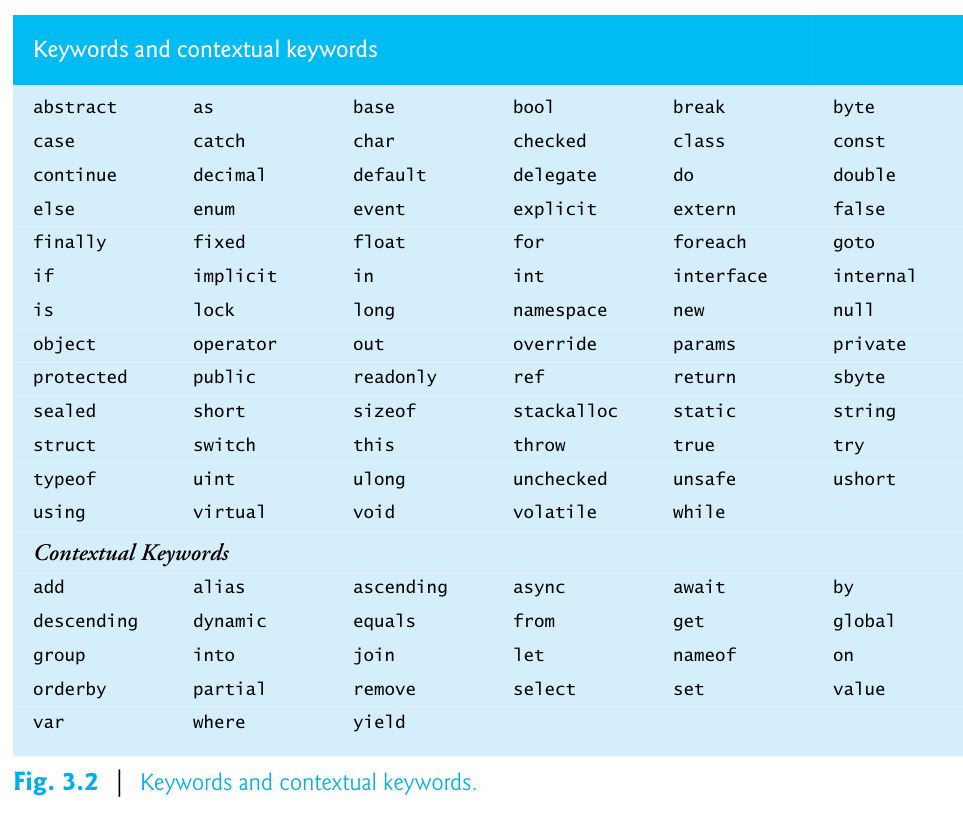
\includegraphics[width=\textwidth]{images/fig3_02_keywords_table.png}
      {\centering\scriptsize \textbf{Bảng 77 từ khóa chuẩn C\# (Hình 3.2)}\par}
      \vspace{-2mm}
      \begin{alertblock}{\textbf{Quy tắc định danh:}}
        Không được dùng từ khóa C\# (\texttt{class}, \texttt{static}, \texttt{void}...) làm tên biến/tên lớp, và không được bắt đầu bằng chữ số!
      \end{alertblock}
    \end{column}
  \end{columns}
\end{frame}

% ==============================================================================
% SLIDE 9: PHƯƠNG THỨC MAIN & CẶP NGOẶC NHỌN
% ==============================================================================
\begin{frame}{Điểm Khởi nhập \texttt{static void Main()}, Cặp ngoặc nhọn \& Khối lệnh}
  \begin{columns}[T]
    \begin{column}{0.48\textwidth}
      \begin{block}{\textbf{Phương thức \texttt{Main()}}}
        \begin{itemize}\small
          \item \textbf{Cửa ngõ thực thi (Entry Point):} Máy ảo CLR luôn tìm và bắt đầu thực thi chương trình C\# từ phương thức \texttt{Main}.
          \item Từ khóa \texttt{static}: Cho phép CLR gọi thực thi phương thức mà không cần tạo đối tượng của lớp trước.
          \item Từ khóa \texttt{void}: Báo hiệu phương thức này không trả về bất kỳ dữ liệu nào khi hoàn tất tác vụ.
          \item Cặp ngoặc đơn \texttt{()}: Chứa danh sách tham số (trong Welcome1 không có tham số).
        \end{itemize}
      \end{block}
    \end{column}

    \begin{column}{0.48\textwidth}
      \begin{block}{\textbf{Cặp ngoặc nhọn \texttt{\{\}} \& Khối lệnh (Block)}}
        \begin{itemize}\small
          \item Dấu mở ngoặc nhọn \texttt{\{}: Đánh dấu bắt đầu phần thân (body) của một lớp hoặc một phương thức.
          \item Dấu đóng ngoặc nhọn \texttt{\}}: Đánh dấu kết thúc phần thân.
          \item Luôn phải xuất hiện theo từng cặp tương ứng khớp nhau (\textbf{matching pairs}).
        \end{itemize}
      \end{block}

      \begin{exampleblock}{\textbf{Quy chuẩn thụt lề (Indentation):}}
        Thụt vào 1 tab (3 hoặc 4 dấu cách) cho mỗi cấp độ khối lệnh bên trong để mã nguồn rõ ràng, chuyên nghiệp.
      \end{exampleblock}
    \end{column}
  \end{columns}
\end{frame}

% ==============================================================================
% SLIDE 10: LỆNH XUẤT DỮ LIỆU CONSOLE.WRITELINE
% ==============================================================================
\begin{frame}[fragile]{Xuất Dữ liệu ra Màn hình: \texttt{Console.WriteLine()}}
  \begin{tcolorbox}[colback=CodeBg,colframe=UniBlue,title=\textbf{Cú pháp câu lệnh xuất chuẩn C\#},fonttitle=\small\bfseries]
    \centering
    \Large \texttt{Console.WriteLine("Welcome to C\# Programming!");}
  \end{tcolorbox}

  \begin{columns}[T]
    \begin{column}{0.48\textwidth}
      \begin{block}{\textbf{Giải phẫu câu lệnh:}}
        \begin{itemize}\small
          \item \textbf{\texttt{Console}:} Lớp đại diện cho cửa sổ dòng lệnh chuẩn của hệ điều hành.
          \item \textbf{Toán tử chấm (\texttt{.}):} Toán tử truy cập thành viên, dùng để gọi phương thức \texttt{WriteLine} của lớp \texttt{Console}.
          \item \textbf{Đối số (Argument):} Chuỗi ký tự nằm trong cặp nháy kép \texttt{"..."} được truyền vào cho phương thức in ra màn hình.
          \item \textbf{Cơ chế hoạt động:} In chuỗi văn bản ra cửa sổ console và \textbf{tự động đưa con trỏ xuống đầu dòng kế tiếp}.
        \end{itemize}
      \end{block}
    \end{column}

    \begin{column}{0.48\textwidth}
      \begin{alertblock}{\textbf{Dấu chấm phẩy (\texttt{;}) -- Dấu hiệu kết thúc câu lệnh}}
        \begin{itemize}\small
          \item Mọi câu lệnh đơn trong C\# đều \textbf{bắt buộc phải kết thúc bằng dấu chấm phẩy \texttt{;}}.
          \item Thiếu dấu chấm phẩy là lỗi cú pháp sơ đẳng phổ biến nhất của người mới học lập trình!
        \end{itemize}
      \end{alertblock}

      \begin{exampleblock}{\textbf{Chuỗi ký tự (String Literal):}}
        Một dãy các ký tự nằm trong cặp nháy kép \texttt{"..."}. Nháy kép không được in ra màn hình, chỉ có nội dung bên trong được hiển thị.
      \end{exampleblock}
    \end{column}
  \end{columns}
\end{frame}

% ==============================================================================
% SLIDE 11: QUY TRÌNH TẠO CONSOLE APP TRONG VISUAL STUDIO
% ==============================================================================
\begin{frame}{Thao tác Visual Studio: Khởi tạo Dự án Console Application}
  \begin{columns}[T]
    \begin{column}{0.48\textwidth}
      \centering
      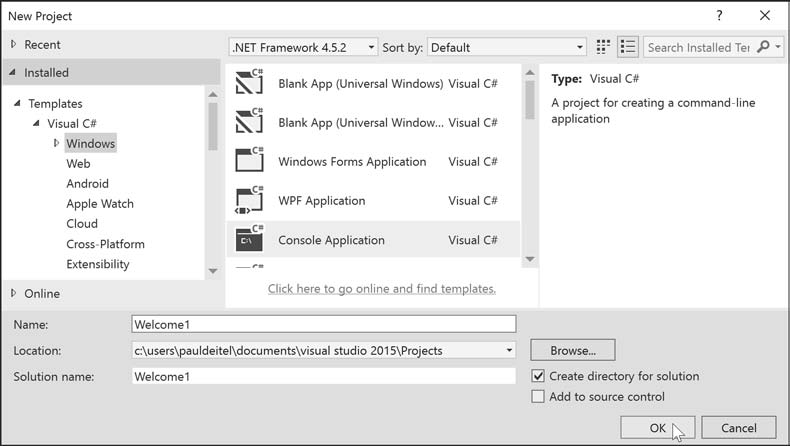
\includegraphics[width=\textwidth]{images/fig3_03_new_console_project.png}
      {\centering\scriptsize \textbf{Chọn Console Application trong New Project (Hình 3.3)}\par}
      \begin{itemize}\scriptsize
        \item Vào \textbf{File $\to$ New $\to$ Project...} (hoặc Ctrl+Shift+N).
        \item Chọn mẫu: \textbf{Visual C\# $\to$ Windows $\to$ Console Application}.
        \item Đặt tên dự án: \texttt{Welcome1}, chọn đường dẫn lưu tệp.
      \end{itemize}
    \end{column}

    \begin{column}{0.48\textwidth}
      \centering
      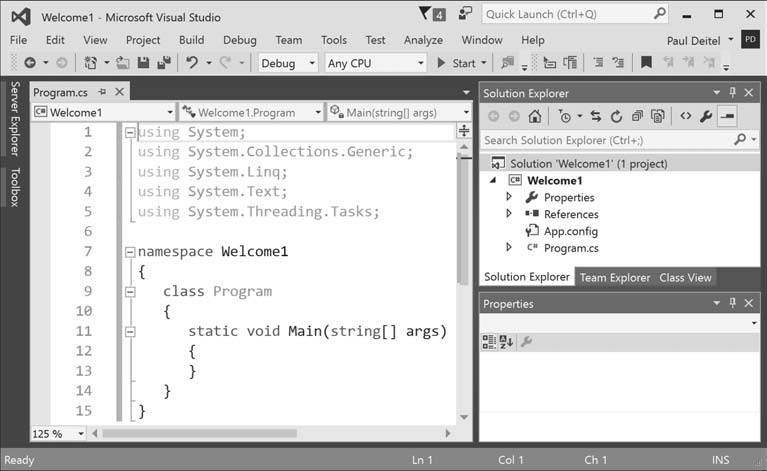
\includegraphics[width=\textwidth]{images/fig3_04_ide_console_app.png}
      {\centering\scriptsize \textbf{Không gian soạn thảo mã Console App (Hình 3.4)}\par}
      \begin{itemize}\scriptsize
        \item IDE tự động sinh tệp mã nguồn mẫu \texttt{Program.cs}.
        \item Đổi tên tệp thành \texttt{Welcome1.cs} trong Solution Explorer (bấm Yes khi IDE hỏi đổi tên lớp).
        \item Khung soạn thảo hỗ trợ đánh số dòng (\textit{Line Numbers}) và tô màu cú pháp.
      \end{itemize}
    \end{column}
  \end{columns}
\end{frame}

% ==============================================================================
% SLIDE 12: TRỢ THỦ INTELLISENSE & PARAMETER INFO
% ==============================================================================
\begin{frame}{Trợ thủ Lập trình: Tính năng IntelliSense \& Parameter Info}
  \begin{columns}[T]
    \begin{column}{0.48\textwidth}
      \centering
      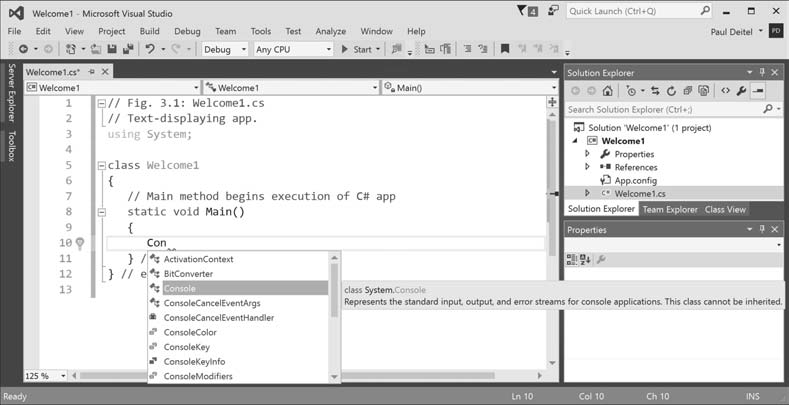
\includegraphics[width=0.85\textwidth]{images/fig3_05_intellisense_typing.png}\\
      \vspace{1mm}
      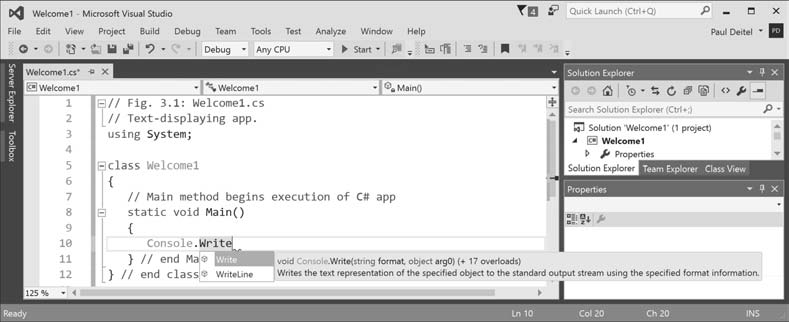
\includegraphics[width=0.85\textwidth]{images/fig3_06_intellisense_members.png}
      {\centering\scriptsize \textbf{Cửa sổ IntelliSense gợi ý tự động (Hình 3.5, 3.6)}\par}
    \end{column}

    \begin{column}{0.48\textwidth}
      \begin{block}{\textbf{Tính năng IntelliSense (Ctrl + Space)}}
        \begin{itemize}\small
          \item Tự động hoàn thành mã nguồn khi bạn gõ vài ký tự đầu (ví dụ: gõ \texttt{Con} $\to$ nhấn \texttt{Tab} để chọn \texttt{Console}).
          \item Hiển thị danh sách tất cả thuộc tính, phương thức khả dụng kèm mô tả ngắn.
        \end{itemize}
      \end{block}

      \centering
      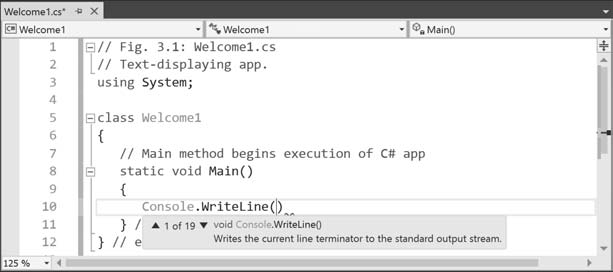
\includegraphics[width=0.9\textwidth]{images/fig3_07_parameter_info.png}
      {\centering\scriptsize \textbf{Cửa sổ Parameter Info (Hình 3.7)}\par}
      \begin{exampleblock}{\textbf{Parameter Info Tooltip:}}
        \small Khi gõ dấu mở ngoặc đơn \texttt{(}, IDE hiển thị số lượng và kiểu dữ liệu của các tham số được hỗ trợ.
      \end{exampleblock}
    \end{column}
  \end{columns}
\end{frame}

% ==============================================================================
% SLIDE 13: BIÊN DỊCH VÀ CHẠY THỬ ỨNG DỤNG
% ==============================================================================
\begin{frame}{Biên dịch và Chạy thử: Run Mode (Phím tắt Ctrl + F5)}
  \begin{columns}[T]
    \begin{column}{0.50\textwidth}
      \begin{block}{\textbf{Quy trình Thực thi Ứng dụng Console:}}
        \begin{enumerate}\small
          \item \textbf{Phím tắt thực thi:} Nhấn \textbf{Ctrl + F5} (\textit{Start Without Debugging}).
          \item \textbf{Cơ chế biên dịch:} Trình biên dịch C\# kiểm tra cú pháp và sinh tệp thực thi \texttt{Welcome1.exe} trong thư mục \texttt{bin/Debug/}.
          \item \textbf{Khởi chạy:} Hệ điều hành mở cửa sổ Command Prompt màu đen, thực thi ứng dụng và in kết quả.
        \end{enumerate}
      \end{block}

      \begin{alertblock}{\textbf{Tại sao dùng Ctrl+F5 thay vì F5?}}
        \small Nhấn F5 (Debug) sẽ đóng cửa sổ Console ngay khi hoàn thành, khiến ta không kịp đọc kết quả. \textbf{Ctrl+F5} sẽ giữ màn hình và hiển thị dòng chữ: \textit{"Press any key to continue . . ."}.
      \end{alertblock}
    \end{column}

    \begin{column}{0.46\textwidth}
      \centering
      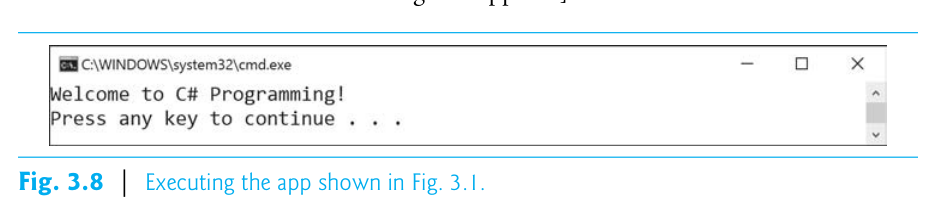
\includegraphics[width=\textwidth]{images/fig3_08_executing_welcome1.png}
      {\centering\scriptsize \textbf{Màn hình thực thi Welcome1.exe trong Command Prompt (Hình 3.8)}\par}
      \vspace{2mm}
      \begin{exampleblock}{\textbf{Kết quả mong đợi:}}
        \ttfamily\small
        Welcome to C\# Programming!\\
        Press any key to continue . . .
      \end{exampleblock}
    \end{column}
  \end{columns}
\end{frame}

% ==============================================================================
% SLIDE 14: LỖI CÚ PHÁP & CỬA SỔ ERROR LIST
% ==============================================================================
\begin{frame}{Xử lý Lỗi Biên dịch: Syntax Errors \& Cửa sổ Error List}
  \begin{columns}[T]
    \begin{column}{0.55\textwidth}
      \centering
      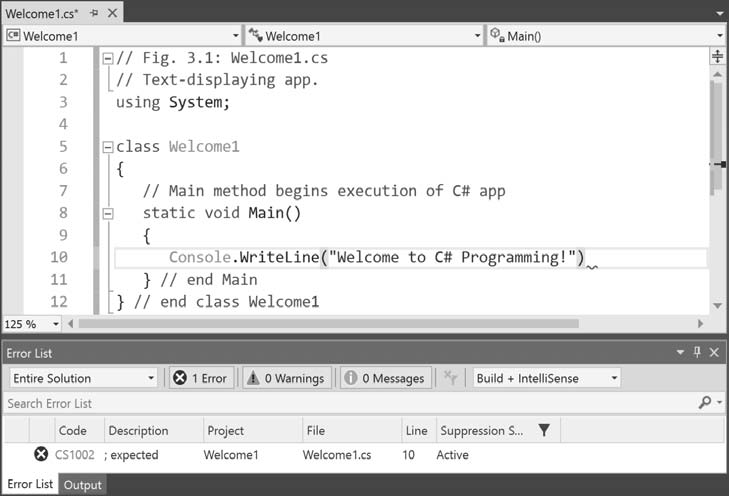
\includegraphics[width=\textwidth]{images/fig3_09_syntax_error_ide.png}
      {\centering\scriptsize \textbf{Gạch lượn sóng đỏ và cửa sổ Error List (Hình 3.9)}\par}
    \end{column}

    \begin{column}{0.42\textwidth}
      \begin{alertblock}{\textbf{1. Lỗi cú pháp (Syntax Error)}}
        \begin{itemize}\small
          \item Vi phạm quy tắc ngữ pháp của C\# (thiếu dấu \texttt{;}, sai tên lớp, thừa ngoặc...).
          \item IDE đánh dấu bằng \textbf{đường gợn sóng đỏ} (\textit{red squiggly line}) ngay dưới vị trí lỗi.
        \end{itemize}
      \end{alertblock}

      \begin{block}{\textbf{2. Cửa sổ Error List}}
        \begin{itemize}\small
          \item Liệt kê mã lỗi (\texttt{CS1002}), mô tả lỗi, tệp tin và số dòng gặp sự cố.
          \item \textbf{Mẹo kỹ sư:} Nhấp đúp chuột vào dòng lỗi trong Error List sẽ tự động nhảy con trỏ tới đúng vị trí cần sửa!
        \end{itemize}
      \end{block}
    \end{column}
  \end{columns}
\end{frame}

% ==============================================================================
% SLIDE 15: CODE STUDY 2: WELCOME2.CS (WRITE VS WRITELINE)
% ==============================================================================
\begin{frame}[fragile]{Biến thể Xuất Dữ liệu: \texttt{Console.Write} vs \texttt{WriteLine}}
  \begin{columns}[T]
    \begin{column}{0.55\textwidth}
      \begin{tcolorbox}[colback=CodeBg,colframe=UniBlue,title=\textbf{Welcome2.cs (Fig. 3.10)},fonttitle=\small\bfseries]
\begin{lstlisting}
// Fig. 3.10: Welcome2.cs
// Displaying one line of text with multiple statements.
using System;

class Welcome2
{
   static void Main()
   {
      Console.Write("Welcome to ");
      Console.WriteLine("C# Programming!");
   } // end Main
} // end class Welcome2
\end{lstlisting}
      \end{tcolorbox}
    \end{column}

    \begin{column}{0.43\textwidth}
      \begin{block}{\textbf{Phân biệt then chốt:}}
        \begin{itemize}\small
          \item \textbf{\texttt{Console.Write()}:} In chuỗi ra màn hình nhưng \textbf{giữ nguyên con trỏ ở cùng một dòng}.
          \item \textbf{\texttt{Console.WriteLine()}:} In chuỗi ra màn hình và \textbf{đưa con trỏ xuống dòng tiếp theo}.
        \end{itemize}
      \end{block}

      \begin{exampleblock}{\textbf{Kết quả đầu ra:}}
        Hai lệnh xuất nối tiếp nhau trên cùng một dòng duy nhất:
        \begin{tcolorbox}[colback=UniDark,colframe=black]
          \color{white}\ttfamily\small
          Welcome to C\# Programming!
        \end{tcolorbox}
      \end{exampleblock}
    \end{column}
  \end{columns}
\end{frame}

% ==============================================================================
% SLIDE 16: CHECKPOINT 1 & THỰC HÀNH TIẾT 1
% ==============================================================================
\begin{frame}{Checkpoint 1: Kiểm tra Nhanh \& Thực hành Tiết 1}
  \begin{block}{\textbf{Câu hỏi 1: Lệnh nào sau đây hợp lệ để in thông điệp và xuống dòng?}}
    \begin{itemize}
      \item[A.] \texttt{console.writeline("Hello");}
      \item[B.] \texttt{Console.WriteLine("Hello");} \textbf{(Đáp án Đúng -- PascalCase chuẩn)}
      \item[C.] \texttt{Console.writeline("Hello")}
      \item[D.] \texttt{System.out.println("Hello");}
    \end{itemize}
  \end{block}

  \begin{alertblock}{\textbf{Câu hỏi 2: Điều gì xảy ra nếu quên dấu chấm phẩy \texttt{;} ở cuối câu lệnh?}}
    Trình biên dịch báo lỗi cú pháp \textbf{CS1002: ; expected} tại cửa sổ Error List và ngăn chặn biên dịch.
  \end{alertblock}

  \begin{exampleblock}{\textbf{Hands-on Lab 1 (Phòng máy -- 10 phút):}}
    Mở Visual Studio $\to$ Tạo Console Application \texttt{Welcome1} $\to$ Gõ mã nguồn $\to$ Chạy thử với \textbf{Ctrl+F5} $\to$ Thử thay bằng \texttt{Console.Write} và quan sát vị trí con trỏ!
  \end{exampleblock}
\end{frame}

% ==============================================================================
% SLIDE 17: TIẾT 2 DIVIDER
% ==============================================================================
\begin{frame}[plain]
  \vfill
  \centering
  \begin{beamercolorbox}[sep=8pt,center,shadow=true,rounded=true]{palette secondary}
    {\Huge \textbf{TIẾT 2}}\\[2mm]
    {\Large \textbf{KÝ TỰ THOÁT, NỘI SUY CHUỖI, BIẾN SỐ, BỘ NHỚ RAM \& PHÉP TOÁN SỐ HỌC}}
  \end{beamercolorbox}
  \vfill
\end{frame}

% ==============================================================================
% SLIDE 18: CODE STUDY 3: WELCOME3.CS
% ==============================================================================
\begin{frame}[fragile]{Xuất Nhiều Dòng Bằng Một Lệnh: \texttt{Welcome3.cs}}
  \begin{columns}[T]
    \begin{column}{0.55\textwidth}
      \begin{tcolorbox}[colback=CodeBg,colframe=CSharpPurple,title=\textbf{Welcome3.cs (Fig. 3.11)},fonttitle=\small\bfseries]
\begin{lstlisting}
// Fig. 3.11: Welcome3.cs
// Displaying multiple lines with a single statement.
using System;

class Welcome3
{
   static void Main()
   {
      Console.WriteLine("Welcome\nto\nC#\nProgramming!");
   } // end Main
} // end class Welcome3
\end{lstlisting}
      \end{tcolorbox}
    \end{column}

    \begin{column}{0.43\textwidth}
      \begin{block}{\textbf{Cơ chế Ký tự Thoát \texttt{\textbackslash n}:}}
        \begin{itemize}\small
          \item Ký tự gạch chéo ngược (\texttt{\textbackslash}) gọi là \textbf{ký tự thoát (Escape character)}.
          \item Kết hợp với ký tự đi liền kề tạo thành một \textbf{dãy ký tự thoát (Escape Sequence)}.
          \item \texttt{\textbackslash n} đại diện cho lệnh xuống dòng (\textit{Newline}), chuyển con trỏ sang dòng mới.
        \end{itemize}
      \end{block}

      \begin{exampleblock}{\textbf{Kết quả in ra 4 dòng:}}
        \begin{tcolorbox}[colback=UniDark,colframe=black]
          \color{white}\ttfamily\small
          Welcome\\
          to\\
          C\#\\
          Programming!
        \end{tcolorbox}
      \end{exampleblock}
    \end{column}
  \end{columns}
\end{frame}

% ==============================================================================
% SLIDE 19: BẢNG KÝ TỰ THOÁT THÔNG DỤNG (FIG 3.12)
% ==============================================================================
\begin{frame}{Bảng Tra cứu Ký tự Thoát Thông dụng (Escape Sequences)}
  \begin{columns}[T]
    \begin{column}{0.55\textwidth}
      \centering
      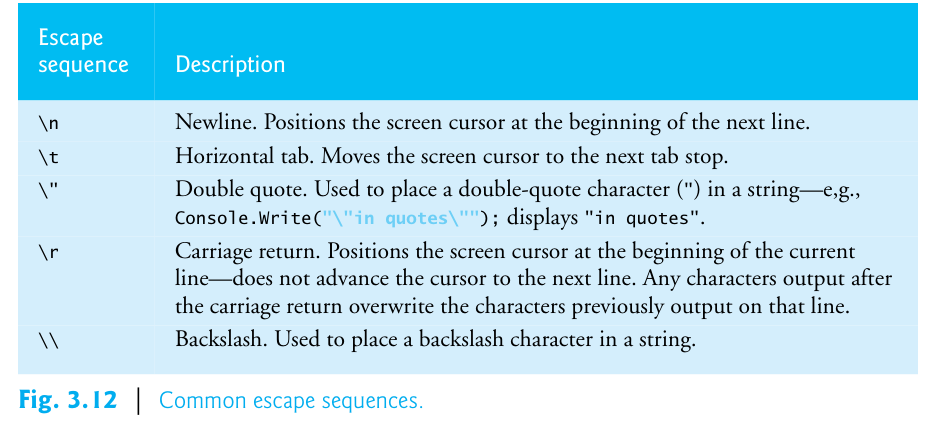
\includegraphics[width=\textwidth]{images/fig3_12_escape_sequences_table.png}
      {\centering\scriptsize \textbf{Bảng các ký tự thoát thông dụng trong C\# (Hình 3.12)}\par}
    \end{column}

    \begin{column}{0.43\textwidth}
      \begin{block}{\textbf{Phân tích các Ký tự Tiêu biểu:}}
        \begin{itemize}\small
          \item \textbf{\texttt{\textbackslash n} (Newline):} Đưa con trỏ xuống đầu dòng kế tiếp.
          \item \textbf{\texttt{\textbackslash t} (Horizontal Tab):} Đẩy con trỏ sang điểm dừng tab tiếp theo (thường là 4 hoặc 8 khoảng trắng).
          \item \textbf{\texttt{\textbackslash r} (Carriage Return):} Đưa con trỏ về đầu dòng hiện tại.
          \item \textbf{\texttt{\textbackslash\textbackslash} (Backslash):} In chính ký tự gạch chéo ngược \texttt{\textbackslash}.
          \item \textbf{\texttt{\textbackslash"} (Double Quote):} In dấu nháy kép \texttt{"} bên trong chuỗi mà không bị nhầm là kết thúc chuỗi.
        \end{itemize}
      \end{block}
      \begin{exampleblock}{\textbf{Ví dụ in nháy kép:}}
        \texttt{Console.WriteLine("\textbackslash"C\#\textbackslash"");} $\to$ in ra \texttt{"C\#"}
      \end{exampleblock}
    \end{column}
  \end{columns}
\end{frame}

% ==============================================================================
% SLIDE 20: STRING INTERPOLATION C# 6 (FIG 3.13)
% ==============================================================================
\begin{frame}[fragile]{Tính năng Hiện đại C\# 6: Nội suy Chuỗi (String Interpolation)}
  \begin{columns}[T]
    \begin{column}{0.55\textwidth}
      \begin{tcolorbox}[colback=CodeBg,colframe=CSharpPurple,title=\textbf{Welcome4.cs (Fig. 3.13)},fonttitle=\small\bfseries]
\begin{lstlisting}
// Fig. 3.13: Welcome4.cs
// Inserting content into a string with string interpolation.
using System;

class Welcome4
{
   static void Main()
   {
      string person = "Paul"; // variable that stores the name Paul
      Console.WriteLine($"Welcome to C# Programming, {person}!");
   } // end Main
} // end class Welcome4
\end{lstlisting}
      \end{tcolorbox}
    \end{column}

    \begin{column}{0.43\textwidth}
      \begin{block}{\textbf{Cú pháp Nội suy Chuỗi: \texttt{\$"..."}}}
        \begin{itemize}\small
          \item Bắt đầu chuỗi bằng ký tự đô-la (\texttt{\$}) đặt ngay trước dấu nháy kép mở.
          \item Nhúng trực tiếp biến hoặc biểu thức vào bên trong cặp ngoặc nhọn \texttt{\{biểu\_thức\}}.
          \item Giá trị của biểu thức sẽ được tự động tính toán và chèn vào đúng vị trí đó!
        \end{itemize}
      \end{block}

      \begin{exampleblock}{\textbf{Ưu thế so với cách cũ:}}
        Cách cũ: \texttt{"Welcome " + person + "!"}\\
        Nội suy C\# 6: \texttt{\$"Welcome \{person\}!"}\\
        $\to$ \textbf{Ngắn gọn, trực quan, chạy nhanh hơn và hạn chế lỗi cú pháp!}
      \end{exampleblock}
    \end{column}
  \end{columns}
\end{frame}

% ==============================================================================
% SLIDE 21: CODE STUDY 4: ADDITION.CS
% ==============================================================================
\begin{frame}[fragile]{Ứng dụng Nhập liệu \& Tính toán: \texttt{Addition.cs}}
  \begin{columns}[T]
    \begin{column}{0.55\textwidth}
      \begin{tcolorbox}[colback=CodeBg,colframe=UniNavy,title=\textbf{Addition.cs (Fig. 3.14)},fonttitle=\small\bfseries]
\begin{lstlisting}
using System;

class Addition
{
   static void Main()
   {
      int number1; // declare first number to add
      int number2; // declare second number to add
      int sum;     // declare sum of number1 and number2

      Console.Write("Enter first integer: ");
      number1 = int.Parse(Console.ReadLine());

      Console.Write("Enter second integer: ");
      number2 = int.Parse(Console.ReadLine());

      sum = number1 + number2; // add numbers
      Console.WriteLine($"Sum is {sum}"); // display sum
   } // end Main
} // end class Addition
\end{lstlisting}
      \end{tcolorbox}
    \end{column}

    \begin{column}{0.43\textwidth}
      \begin{tcolorbox}[colback=UniDark,colframe=black,title=\textbf{Màn hình Console Tương tác},fonttitle=\scriptsize\bfseries]
        \color{white}\ttfamily\small
        Enter first integer: \textbf{45}\\
        Enter second integer: \textbf{72}\\
        Sum is 117
      \end{tcolorbox}

      \begin{exampleblock}{\textbf{Quy trình 3 Giai đoạn:}}
        \begin{enumerate}\small
          \item \textbf{Input:} Nhắc người dùng gõ 2 số từ bàn phím.
          \item \textbf{Process:} Chuyển chuỗi thành số và cộng: \texttt{sum = number1 + number2}.
          \item \textbf{Output:} In kết quả tổng ra màn hình bằng nội suy chuỗi.
        \end{enumerate}
      \end{exampleblock}
    \end{column}
  \end{columns}
\end{frame}

% ==============================================================================
% SLIDE 22: KHAI BÁO BIẾN & KIỂU DỮ LIỆU INT
% ==============================================================================
\begin{frame}{Khai báo Biến (Variable Declaration) \& Kiểu số nguyên \texttt{int}}
  \begin{columns}[T]
    \begin{column}{0.48\textwidth}
      \begin{block}{\textbf{1. Biến (Variable) là gì?}}
        \begin{itemize}\small
          \item Một vùng nhớ trong RAM máy tính được đặt tên để lưu trữ giá trị dữ liệu cho chương trình sử dụng.
          \item Mọi biến trong C\# \textbf{bắt buộc phải được khai báo tên và kiểu dữ liệu} trước khi sử dụng.
        \end{itemize}
      \end{block}

      \begin{exampleblock}{\textbf{Cú pháp khai báo:}}
        \texttt{int number1;}\\
        \texttt{int number2, sum;} // khai báo nhiều biến cùng kiểu
      \end{exampleblock}
    \end{column}

    \begin{column}{0.48\textwidth}
      \begin{block}{\textbf{2. Kiểu dữ liệu \texttt{int}}}
        \begin{itemize}\small
          \item Đại diện cho số nguyên (Integer) trong khoảng từ $-2,147,483,648$ đến $+2,147,483,647$ (chiếm 32-bit = 4 bytes trong RAM).
          \item Không chứa phần thập phân (như $-5, 0, 45, 100$).
        \end{itemize}
      \end{block}

      \begin{exampleblock}{\textbf{Quy ước đặt tên biến (camelCase):}}
        Chữ cái đầu viết thường, các từ tiếp theo viết hoa chữ cái đầu: \texttt{number1}, \texttt{totalScore}, \texttt{itemPrice}.
      \end{exampleblock}
    \end{column}
  \end{columns}
\end{frame}

% ==============================================================================
% SLIDE 23: NHẬP DỮ LIỆU BÀN PHÍM & INT.PARSE
% ==============================================================================
\begin{frame}[fragile]{Nhập Liệu từ Bàn phím: \texttt{Console.ReadLine()} \& \texttt{int.Parse()}}
  \begin{tcolorbox}[colback=CodeBg,colframe=UniBlue,title=\textbf{Cú pháp nhập và chuyển đổi kiểu dữ liệu},fonttitle=\small\bfseries]
    \centering
    \Large \texttt{number1 = int.Parse(Console.ReadLine());}
  \end{tcolorbox}

  \begin{columns}[T]
    \begin{column}{0.48\textwidth}
      \begin{block}{\textbf{Bước 1: \texttt{Console.ReadLine()}}}
        \begin{itemize}\small
          \item Tạm dừng chương trình và chờ người dùng gõ ký tự từ bàn phím.
          \item Khi người dùng nhấn phím \textbf{Enter}, phương thức đọc toàn bộ dòng chữ và trả về một đối tượng \textbf{\texttt{string} (chuỗi)}.
          \item Ví dụ gõ \texttt{45} $\to$ nhận về chuỗi \texttt{"45"} (văn bản, không phải số học!).
        \end{itemize}
      \end{block}
    \end{column}

    \begin{column}{0.48\textwidth}
      \begin{block}{\textbf{Bước 2: \texttt{int.Parse()}}}
        \begin{itemize}\small
          \item Nhận vào chuỗi văn bản và \textbf{chuyển đổi (parse)} nó thành giá trị số nguyên \texttt{int}.
          \item Chuỗi \texttt{"45"} $\to$ biến thành số nguyên \texttt{45} để có thể thực hiện các phép cộng trừ nhân chia.
        \end{itemize}
      \end{block}

      \begin{alertblock}{\textbf{Cảnh báo ngoại lệ FormatException:}}
        Nếu người dùng gõ chữ cái (ví dụ \texttt{"abc"}), lệnh \texttt{int.Parse} sẽ báo lỗi \textit{FormatException} vì không thể chuyển thành số!
      \end{alertblock}
    \end{column}
  \end{columns}
\end{frame}

% ==============================================================================
% SLIDE 24: TOÁN TỬ GÁN GIÁ TRỊ (=)
% ==============================================================================
\begin{frame}[fragile]{Toán tử Gán Giá trị (\texttt{=}) \& Luồng Thực thi}
  \begin{tcolorbox}[colback=CodeBg,colframe=UniNavy,title=\textbf{Câu lệnh gán: Tính toán vế phải và lưu vào vế trái},fonttitle=\small\bfseries]
    \centering
    \Large \texttt{sum = number1 + number2;}
  \end{tcolorbox}

  \begin{columns}[T]
    \begin{column}{0.48\textwidth}
      \begin{block}{\textbf{Cơ chế thực thi: Từ Phải sang Trái ($\leftarrow$)}}
        \begin{enumerate}\small
          \item \textbf{Bước 1 (Tính toán vế phải):} Lấy giá trị trong ô nhớ \texttt{number1} (45) cộng với giá trị trong ô nhớ \texttt{number2} (72) $\to$ kết quả tạm thời là \textbf{117}.
          \item \textbf{Bước 2 (Gán vào vế trái):} Toán tử gán \texttt{=} sao chép giá trị 117 và đặt vào ô nhớ được đặt tên là \textbf{\texttt{sum}}.
        \end{enumerate}
      \end{block}
    \end{column}

    \begin{column}{0.48\textwidth}
      \begin{alertblock}{\textbf{Quy tắc vế trái (L-value):}}
        Vế trái của toán tử \texttt{=} bắt buộc phải là một tên biến (vùng nhớ có thể nhận dữ liệu). Không thể viết \texttt{number1 + number2 = sum;} hoặc \texttt{45 = number1;}.
      \end{alertblock}

      \begin{exampleblock}{\textbf{Tính chất kết hợp phải (Right-Associative):}}
        Các câu lệnh gán liên tiếp \texttt{a = b = c = 0;} sẽ được thực hiện từ phải sang trái: \texttt{c = 0}, sau đó \texttt{b = c}, sau đó \texttt{a = b}.
      \end{exampleblock}
    \end{column}
  \end{columns}
\end{frame}

% ==============================================================================
% SLIDE 25: BẢN CHẤT BỘ NHỚ RAM (FIG 3.15, 3.16)
% ==============================================================================
\begin{frame}{Bản chất Bộ nhớ Máy tính (Memory Concepts): Ô nhớ RAM}
  \begin{columns}[T]
    \begin{column}{0.48\textwidth}
      \centering
      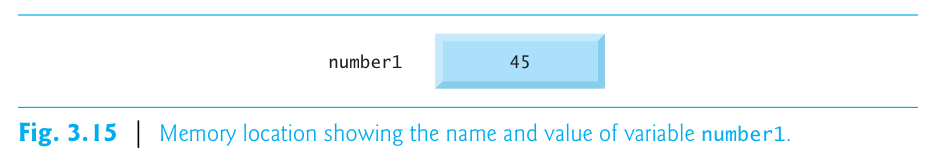
\includegraphics[width=\textwidth]{images/fig3_15_memory_number1.png}
      {\centering\scriptsize \textbf{Ô nhớ sau khi đọc number1 = 45 (Hình 3.15)}\par}
      \vspace{2mm}
      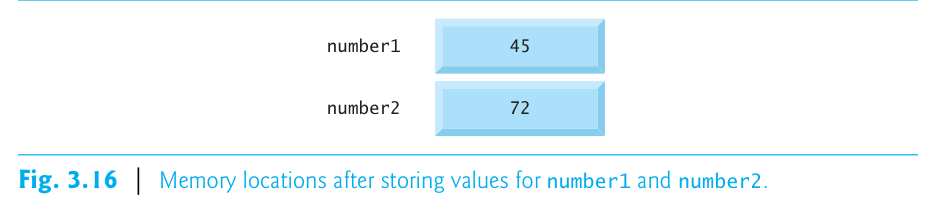
\includegraphics[width=\textwidth]{images/fig3_16_memory_number2.png}
      {\centering\scriptsize \textbf{Ô nhớ sau khi đọc number2 = 72 (Hình 3.16)}\par}
    \end{column}

    \begin{column}{0.48\textwidth}
      \begin{block}{\textbf{Cấu trúc một Ô nhớ trong RAM:}}
        Mỗi biến trong chương trình tương ứng với một vùng nhớ vật lý gồm 4 yếu tố:
        \begin{itemize}\small
          \item \textbf{Tên biến (Name):} Ví dụ \texttt{number1}, dùng cho lập trình viên tham chiếu.
          \item \textbf{Kiểu dữ liệu (Type):} Ví dụ \texttt{int}, quy định kích thước và cách biểu diễn.
          \item \textbf{Địa chỉ (Address):} Vị trí nhị phân thực tế trong chip RAM do CLR quản lý.
          \item \textbf{Giá trị (Value):} Dữ liệu nhị phân đang được lưu trữ bên trong.
        \end{itemize}
      \end{block}
    \end{column}
  \end{columns}
\end{frame}

% ==============================================================================
% SLIDE 26: ĐỌC KHÔNG PHÁ HỦY VS GHI ĐÈ PHÁ HỦY (FIG 3.17)
% ==============================================================================
\begin{frame}{Cơ chế Đọc Không Phá Hủy vs Ghi Đè Phá Hủy trong RAM}
  \begin{columns}[T]
    \begin{column}{0.48\textwidth}
      \centering
      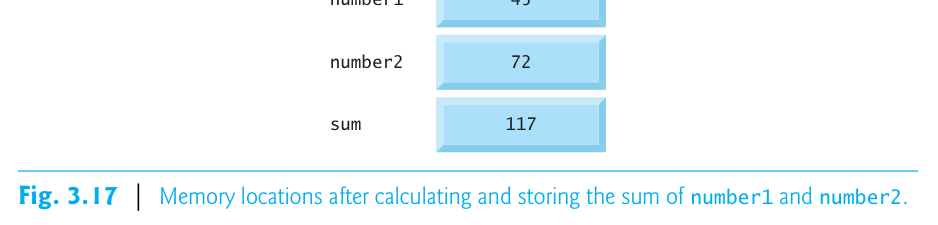
\includegraphics[width=\textwidth]{images/fig3_17_memory_sum.png}
      {\centering\scriptsize \textbf{Các ô nhớ sau khi tính sum = 117 (Hình 3.17)}\par}
      \vspace{2mm}
      \begin{tcolorbox}[colback=UniLightBlue!30,colframe=UniBlue]
        \small Biến \texttt{number1} và \texttt{number2} \textbf{vẫn giữ nguyên giá trị} 45 và 72 sau phép cộng!
      \end{tcolorbox}
    \end{column}

    \begin{column}{0.48\textwidth}
      \begin{exampleblock}{\textbf{1. Đọc Không Phá Hủy (Non-destructive)}}
        \begin{itemize}\small
          \item Khi một biến xuất hiện ở \textbf{vế phải} phép gán (ví dụ: \texttt{number1 + number2}), máy tính chỉ đọc bản sao giá trị của ô nhớ.
          \item Giá trị ban đầu trong ô nhớ được \textbf{bảo toàn nguyên vẹn}, không bị mất đi!
        \end{itemize}
      \end{exampleblock}

      \begin{alertblock}{\textbf{2. Ghi Đè Phá Hủy (Destructive Read-in)}}
        \begin{itemize}\small
          \item Khi một giá trị mới được đưa vào biến ở \textbf{vế trái} (ví dụ: gán vào \texttt{sum}), giá trị mới sẽ \textbf{ghi đè và xóa sổ vĩnh viễn} giá trị cũ trước đó trong ô nhớ.
        \end{itemize}
      \end{alertblock}
    \end{column}
  \end{columns}
\end{frame}

% ==============================================================================
% SLIDE 27: TOÁN TỬ SỐ HỌC C# (FIG 3.18)
% ==============================================================================
\begin{frame}{Các Toán tử Số học Cơ bản trong C\# (Arithmetic Operators)}
  \begin{columns}[T]
    \begin{column}{0.55\textwidth}
      \centering
      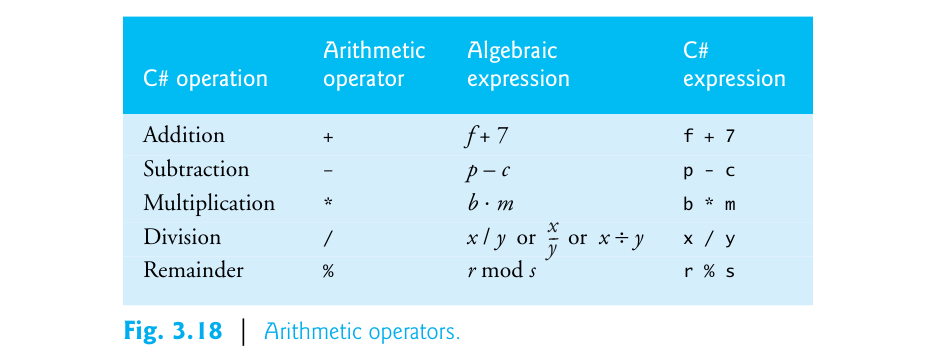
\includegraphics[width=\textwidth]{images/fig3_18_arithmetic_operators.png}
      {\centering\scriptsize \textbf{5 Toán tử số học trong C\# (Hình 3.18)}\par}
    \end{column}

    \begin{column}{0.42\textwidth}
      \begin{block}{\textbf{Ý nghĩa \& Ký hiệu:}}
        \begin{itemize}\small
          \item \textbf{Cộng (\texttt{+}):} \texttt{f + 7}
          \item \textbf{Trừ (\texttt{-}):} \texttt{p - c}
          \item \textbf{Nhân (\texttt{*}):} \texttt{b * m} (không dùng dấu $\times$)
          \item \textbf{Chia (\texttt{/}):} \texttt{x / y} (không dùng dấu $\div$)
          \item \textbf{Chia lấy dư (\texttt{\%}):} \texttt{r \% 5} (toán tử Modulus)
        \end{itemize}
      \end{block}

      \begin{alertblock}{\textbf{Dạng biểu thức phẳng (Straight-Line):}}
        Trong code C\#, mọi biểu thức toán học phải viết trên cùng một dòng ngang, ví dụ: $\frac{a}{b}$ phải viết thành \texttt{a / b}.
      \end{alertblock}
    \end{column}
  \end{columns}
\end{frame}

% ==============================================================================
% SLIDE 28: PHÉP CHIA NGUYÊN & TOÁN TỬ % (MODULUS)
% ==============================================================================
\begin{frame}{Phép Chia Số Nguyên (Truncation) \& Phép Chia Lấy Dư (\%)}
  \begin{columns}[T]
    \begin{column}{0.48\textwidth}
      \begin{alertblock}{\textbf{1. Phép Chia Số Nguyên (Integer Division)}}
        \begin{itemize}\small
          \item Khi chia hai số nguyên (\texttt{int / int}), C\# trả về một số nguyên bằng cách \textbf{vứt bỏ toàn bộ phần thập phân (Truncation)}, hoàn toàn \textbf{không làm tròn}!
          \item \textbf{Ví dụ thực tế:}
            \begin{itemize}\small
              \item \texttt{7 / 4} cho kết quả là \textbf{\texttt{1}} (bỏ mất .75!).
              \item \texttt{17 / 5} cho kết quả là \textbf{\texttt{3}} (bỏ mất .4!).
              \item \texttt{1 / 2} cho kết quả là \textbf{\texttt{0}}!
            \end{itemize}
          \item Muốn có phần thập phân chính xác, ít nhất một toán hạng phải là số thực (\texttt{7.0 / 4} $\to$ \texttt{1.75}).
        \end{itemize}
      \end{alertblock}
    \end{column}

    \begin{column}{0.48\textwidth}
      \begin{exampleblock}{\textbf{2. Toán tử Chia lấy dư (\% Modulus)}}
        \begin{itemize}\small
          \item Cho biết \textbf{phần dư} còn lại sau phép chia số nguyên:
            \begin{itemize}\small
              \item \texttt{7 \% 4} cho kết quả là \textbf{\texttt{3}} ($7 = 4 \times 1 + 3$).
              \item \texttt{17 \% 5} cho kết quả là \textbf{\texttt{2}} ($17 = 5 \times 3 + 2$).
              \item \texttt{8 \% 2} cho kết quả là \textbf{\texttt{0}} ($8 = 2 \times 4 + 0$).
            \end{itemize}
          \item \textbf{Ứng dụng kinh điển trong CNTT:}
            \begin{itemize}\scriptsize
              \item Kiểm tra số chẵn/lẻ: \texttt{x \% 2 == 0} (chẵn).
              \item Kiểm tra bội số: \texttt{x \% y == 0} (x chia hết cho y).
              \item Tách từng chữ số của một số nguyên.
            \end{itemize}
        \end{itemize}
      \end{exampleblock}
    \end{column}
  \end{columns}
\end{frame}

% ==============================================================================
% SLIDE 29: THỨ TỰ ƯU TIÊN TOÁN TỬ SỐ HỌC (FIG 3.19)
% ==============================================================================
\begin{frame}{Quy tắc Thứ tự Ưu tiên Toán tử Số học (Operator Precedence)}
  \begin{columns}[T]
    \begin{column}{0.55\textwidth}
      \centering
      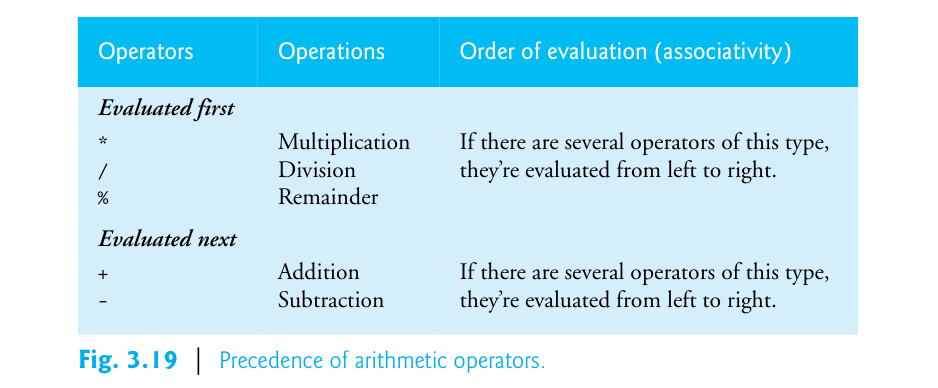
\includegraphics[width=\textwidth]{images/fig3_19_operator_precedence.png}
      {\centering\scriptsize \textbf{Bảng thứ tự ưu tiên của toán tử số học (Hình 3.19)}\par}
    \end{column}

    \begin{column}{0.42\textwidth}
      \begin{block}{\textbf{3 Cấp độ Ưu tiên:}}
        \begin{enumerate}\small
          \item \textbf{Cấp 1 (Cao nhất):} Dấu ngoặc đơn \texttt{()} -- biểu thức trong ngoặc luôn được tính trước nhất!
          \item \textbf{Cấp 2:} Nhân (\texttt{*}), Chia (\texttt{/}), Chia dư (\texttt{\%}).
          \item \textbf{Cấp 3 (Thấp nhất):} Cộng (\texttt{+}) và Trừ (\texttt{-}).
        \end{enumerate}
      \end{block}

      \begin{exampleblock}{\textbf{Tính kết hợp từ trái sang phải:}}
        Khi các toán tử có cùng độ ưu tiên đứng cạnh nhau, C\# thực hiện từ trái qua phải:\\
        \texttt{a * b / c} $\to$ tính \texttt{(a * b)} trước, rồi chia \texttt{c}.
      \end{exampleblock}
    \end{column}
  \end{columns}
\end{frame}

% ==============================================================================
% SLIDE 30: KỸ THUẬT DÙNG DẤU NGOẶC ĐƠN ()
% ==============================================================================
\begin{frame}{Kỹ thuật Sử dụng Dấu ngoặc đơn \texttt{()} \& Tránh Lỗi Nhập nhằng}
  \begin{columns}[T]
    \begin{column}{0.48\textwidth}
      \begin{alertblock}{\textbf{Ví dụ 1: Tính trung bình cộng của 3 số a, b, c}}
        \begin{itemize}\small
          \item \textbf{Viết sai:} \texttt{a + b + c / 3;}\\
          $\to$ Do \texttt{/} ưu tiên hơn \texttt{+}, máy sẽ tính \texttt{a + b + (c / 3)} $\to$ Sai hoàn toàn kết quả!
          \item \textbf{Viết đúng:} \texttt{(a + b + c) / 3;}\\
          $\to$ Cặp ngoặc ép máy tính tổng trước rồi mới chia 3.
        \end{itemize}
      \end{alertblock}
    \end{column}

    \begin{column}{0.48\textwidth}
      \begin{exampleblock}{\textbf{Dấu ngoặc lồng nhau (Nested Parentheses)}}
        \begin{itemize}\small
          \item Cặp ngoặc nằm ở vị trí \textbf{sâu nhất (trong cùng)} sẽ được tính toán đầu tiên:
          \item Ví dụ: \texttt{((a + b) * c) / d}
            \begin{enumerate}\scriptsize
              \item Tính \texttt{(a + b)}
              \item Lấy kết quả nhân với \texttt{c}
              \item Lấy kết quả chia cho \texttt{d}
            \end{enumerate}
          \item \textbf{Lời khuyên Clean Code:} Dùng ngoặc dư thừa hợp lý để biểu thức luôn sáng sủa, không bắt đồng nghiệp phải tra bảng ưu tiên!
        \end{itemize}
      \end{exampleblock}
    \end{column}
  \end{columns}
\end{frame}

% ==============================================================================
% SLIDE 31: CASE STUDY ĐA THỨC BẬC HAI (FIG 3.20)
% ==============================================================================
\begin{frame}{Case Study: Đánh giá Đa thức Bậc hai $y = ax^2 + bx + c$}
  \begin{columns}[T]
    \begin{column}{0.55\textwidth}
      \centering
      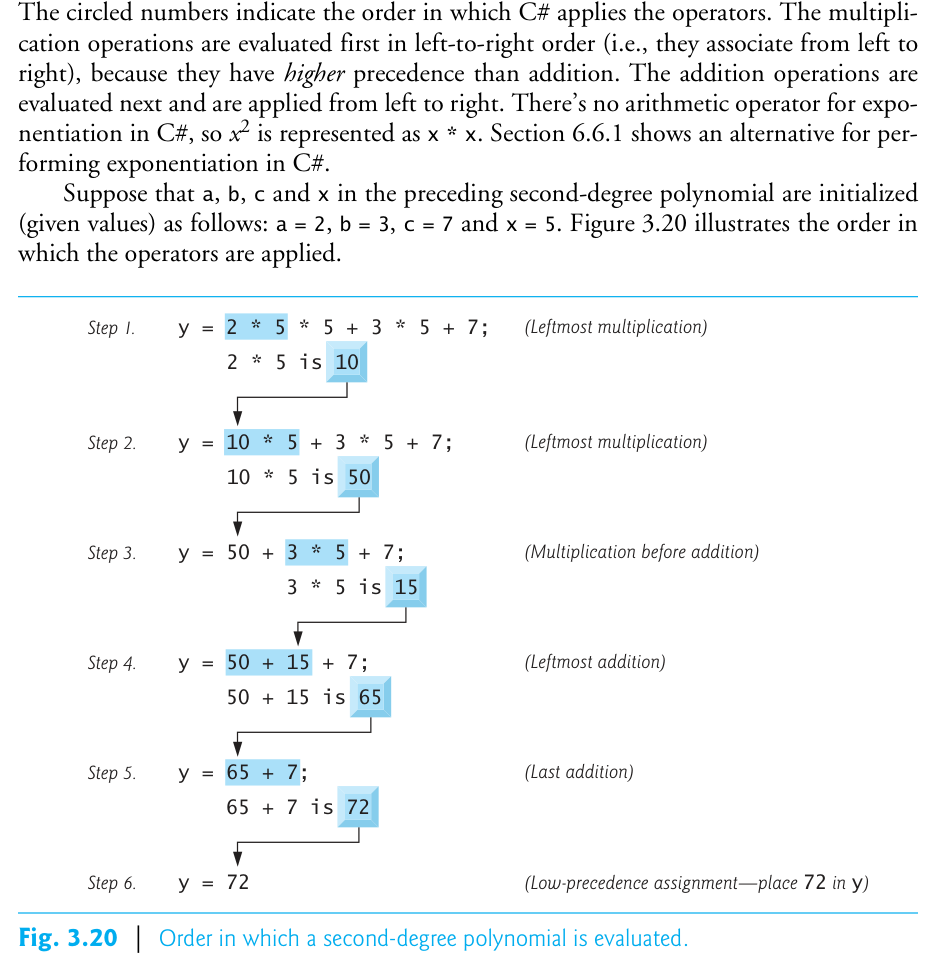
\includegraphics[width=\textwidth]{images/fig3_20_polynomial_evaluation.png}
      {\centering\scriptsize \textbf{Các bước đánh giá biểu thức đa thức bậc hai (Hình 3.20)}\par}
    \end{column}

    \begin{column}{0.42\textwidth}
      \begin{tcolorbox}[colback=CodeBg,colframe=UniNavy,title=\textbf{Biểu thức C\# tương đương},fonttitle=\small\bfseries]
        \centering
        \texttt{y = a * x * x + b * x + c;}
      \end{tcolorbox}

      \begin{block}{\textbf{Giả sử: a=2, b=3, c=7, x=5}}
        \begin{enumerate}\scriptsize
          \item \textbf{Bước 1:} \texttt{2 * 5} = 10
          \item \textbf{Bước 2:} \texttt{10 * 5} = 50 ($ax^2$)
          \item \textbf{Bước 3:} \texttt{3 * 5} = 15 ($bx$)
          \item \textbf{Bước 4:} \texttt{50 + 15} = 65
          \item \textbf{Bước 5:} \texttt{65 + 7} = 72
          \item \textbf{Bước 6:} \texttt{y = 72} (gán giá trị)
        \end{enumerate}
      \end{block}
    \end{column}
  \end{columns}
\end{frame}

% ==============================================================================
% SLIDE 32: CHECKPOINT 2 & THỰC HÀNH TIẾT 2
% ==============================================================================
\begin{frame}{Checkpoint 2: Kiểm tra Nhanh \& Thực hành Tiết 2}
  \begin{block}{\textbf{Câu hỏi 1: Kết quả của biểu thức \texttt{19 \% 5 * 2} trong C\# là bao nhiêu?}}
    \begin{itemize}
      \item[A.] 1.9
      \item[B.] \textbf{8} (Giải thích: \texttt{19 \% 5} = 4, sau đó \texttt{4 * 2} = 8)
      \item[C.] 0
      \item[D.] 4
    \end{itemize}
  \end{block}

  \begin{block}{\textbf{Câu hỏi 2: Kết quả của phép chia số nguyên \texttt{5 / 2} là gì?}}
    Kết quả là \textbf{\texttt{2}} (do C\# vứt bỏ phần thập phân .5).
  \end{block}

  \begin{exampleblock}{\textbf{Hands-on Lab 2 (Phòng máy -- 15 phút):}}
    Tạo dự án \texttt{Addition} $\to$ Khai báo 3 biến \texttt{int} $\to$ Nhập 2 số từ bàn phím bằng \texttt{int.Parse(Console.ReadLine())} $\to$ Tính tổng và in kết quả bằng nội suy chuỗi \texttt{\$"Sum is \{sum\}"}!
  \end{exampleblock}
\end{frame}

% ==============================================================================
% SLIDE 33: TIẾT 3 DIVIDER
% ==============================================================================
\begin{frame}[plain]
  \vfill
  \centering
  \begin{beamercolorbox}[sep=8pt,center,shadow=true,rounded=true]{palette quaternary}
    {\Huge \textbf{TIẾT 3}}\\[2mm]
    {\Large \textbf{CẤU TRÚC RẼ NHÁNH IF, TOÁN TỬ SO SÁNH, COMPARISON \& THỰC HÀNH TỔNG HỢP}}
  \end{beamercolorbox}
  \vfill
\end{frame}

% ==============================================================================
% SLIDE 34: CÂU LỆNH RẼ NHÁNH ĐIỀU KIỆN IF
% ==============================================================================
\begin{frame}[fragile]{Ra Quyết Định trong Phần mềm: Câu lệnh Điều kiện đơn \texttt{if}}
  \begin{columns}[T]
    \begin{column}{0.50\textwidth}
      \begin{block}{\textbf{Nguyên lý Ra quyết định:}}
        \begin{itemize}\small
          \item Cho phép chương trình lựa chọn thực thi hoặc bỏ qua một hành động dựa trên kết quả của một \textbf{điều kiện logic} (True hoặc False).
          \item Cú pháp tổng quát:
\begin{lstlisting}
if (condition)
   statement;
\end{lstlisting}
          \item Nếu điều kiện là \textbf{\texttt{true}}: câu lệnh \texttt{statement} được thực thi.
          \item Nếu điều kiện là \textbf{\texttt{false}}: câu lệnh bị bỏ qua, tiếp tục chạy lệnh kế tiếp.
        \end{itemize}
      \end{block}
    \end{column}

    \begin{column}{0.46\textwidth}
      \begin{tcolorbox}[colback=CodeBg,colframe=UniGreen,title=\textbf{Ví dụ kiểm tra điểm đậu môn},fonttitle=\small\bfseries]
\begin{lstlisting}
if (score >= 50)
   Console.WriteLine("Passed!");
\end{lstlisting}
      \end{tcolorbox}

      \begin{exampleblock}{\textbf{Đặc điểm điều kiện:}}
        Biểu thức điều kiện trong ngoặc đơn \texttt{(condition)} \textbf{bắt buộc phải trả về giá trị kiểu boolean} (\texttt{true} hoặc \texttt{false}). C\# không cho phép dùng số nguyên thay cho boolean như ngôn ngữ C/C++.
      \end{exampleblock}
    \end{column}
  \end{columns}
\end{frame}

% ==============================================================================
% SLIDE 35: BẢNG TOÁN TỬ SO SÁNH (FIG 3.21)
% ==============================================================================
\begin{frame}{Toán tử Quan hệ (Relational) \& Bình đẳng (Equality)}
  \begin{columns}[T]
    \begin{column}{0.55\textwidth}
      \centering
      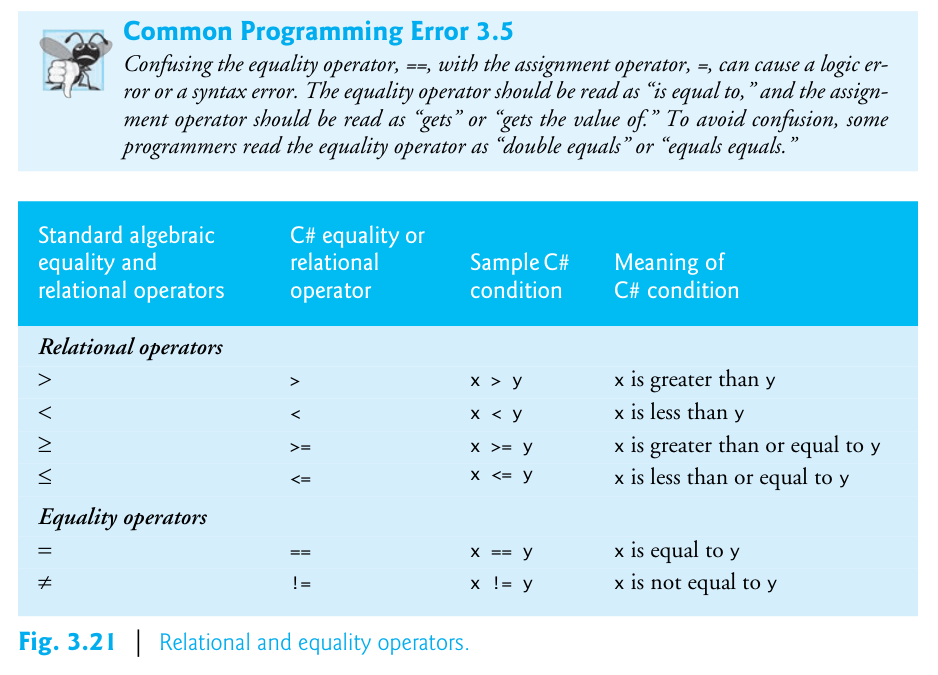
\includegraphics[width=\textwidth]{images/fig3_21_relational_operators.png}
      {\centering\scriptsize \textbf{Các toán tử quan hệ và bình đẳng trong C\# (Hình 3.21)}\par}
    \end{column}

    \begin{column}{0.42\textwidth}
      \begin{block}{\textbf{1. Toán tử Quan hệ (Cùng ưu tiên):}}
        \begin{itemize}\small
          \item \textbf{\texttt{>}} (Lớn hơn): \texttt{x > y}
          \item \textbf{\texttt{<}} (Nhỏ hơn): \texttt{x < y}
          \item \textbf{\texttt{>=}} (Lớn hơn hoặc bằng): \texttt{x >= y}
          \item \textbf{\texttt{<=}} (Nhỏ hơn hoặc bằng): \texttt{x <= y}
        \end{itemize}
      \end{block}

      \begin{block}{\textbf{2. Toán tử Bình đẳng (Ưu tiên thấp hơn):}}
        \begin{itemize}\small
          \item \textbf{\texttt{==}} (Bằng nhau): \texttt{x == y}
          \item \textbf{\texttt{!=}} (Khác nhau / Không bằng): \texttt{x != y}
        \end{itemize}
      \end{block}
    \end{column}
  \end{columns}
\end{frame}

% ==============================================================================
% SLIDE 36: LỖI KINH ĐIỂN 1: PHÂN BIỆT = VÀ ==
% ==============================================================================
\begin{frame}[fragile]{Lỗi Kinh điển \#1: Phân biệt Sống còn giữa \texttt{=} và \texttt{==}}
  \begin{columns}[T]
    \begin{column}{0.48\textwidth}
      \begin{alertblock}{\textbf{Toán tử Gán (\texttt{=})}}
        \begin{itemize}\small
          \item \textbf{Mục đích:} Gán giá trị biểu thức bên phải vào biến bên trái.
          \item \textbf{Cú pháp:} \texttt{x = 7;}
          \item Làm thay đổi giá trị của ô nhớ \texttt{x}.
          \item Không phải là phép so sánh toán học!
        \end{itemize}
      \end{alertblock}
    \end{column}

    \begin{column}{0.48\textwidth}
      \begin{exampleblock}{\textbf{Toán tử So sánh bằng (\texttt{==})}}
        \begin{itemize}\small
          \item \textbf{Mục đích:} Kiểm tra xem 2 vế có bằng nhau hay không.
          \item \textbf{Cú pháp:} \texttt{if (x == 7)}
          \item Trả về \textbf{\texttt{true}} nếu bằng nhau, \textbf{\texttt{false}} nếu khác.
          \item Tuyệt đối \textbf{không làm thay đổi} giá trị của \texttt{x}.
        \end{itemize}
      \end{exampleblock}
    \end{column}
  \end{columns}
  \vspace{2mm}
  \begin{tcolorbox}[colback=UniOrange!10,colframe=UniOrange,title=\textbf{Bẫy cú pháp cần ghi nhớ suốt sự nghiệp kỹ sư:}]
    Trong C\#, nếu viết nhầm \texttt{if (x = 7)}, trình biên dịch sẽ \textbf{chặn ngay lập tức} bằng lỗi: \textit{Cannot implicitly convert type 'int' to 'bool'} (khác với C/C++ sẽ âm thầm gán và gây lỗi logic nghiêm trọng).
  \end{tcolorbox}
\end{frame}

% ==============================================================================
% SLIDE 37: CODE STUDY 5: COMPARISON.CS
% ==============================================================================
\begin{frame}[fragile]{Ứng dụng So sánh Hai Số: \texttt{Comparison.cs}}
  \begin{columns}[T]
    \begin{column}{0.55\textwidth}
      \begin{tcolorbox}[colback=CodeBg,colframe=UniNavy,title=\textbf{Comparison.cs (Fig. 3.22)},fonttitle=\small\bfseries]
\begin{lstlisting}[basicstyle=\ttfamily\tiny]
using System;

class Comparison
{
   static void Main()
   {
      Console.Write("Enter first integer: ");
      int number1 = int.Parse(Console.ReadLine());

      Console.Write("Enter second integer: ");
      int number2 = int.Parse(Console.ReadLine());

      if (number1 == number2)
         Console.WriteLine($"{number1} == {number2}");

      if (number1 != number2)
         Console.WriteLine($"{number1} != {number2}");

      if (number1 < number2)
         Console.WriteLine($"{number1} < {number2}");

      if (number1 > number2)
         Console.WriteLine($"{number1} > {number2}");

      if (number1 <= number2)
         Console.WriteLine($"{number1} <= {number2}");

      if (number1 >= number2)
         Console.WriteLine($"{number1} >= {number2}");
   } // end Main
} // end class Comparison
\end{lstlisting}
      \end{tcolorbox}
    \end{column}

    \begin{column}{0.43\textwidth}
      \centering
      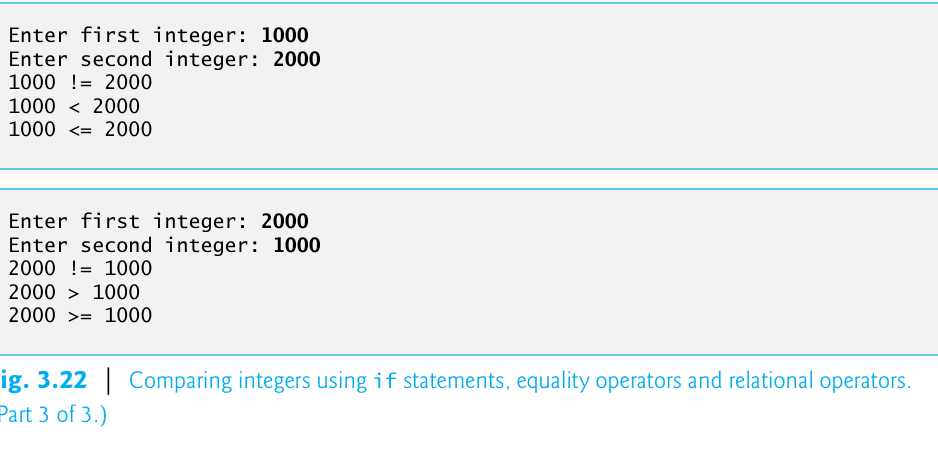
\includegraphics[width=\textwidth]{images/fig3_22_comparison_output.png}
      {\centering\scriptsize \textbf{Màn hình thực thi Comparison (Hình 3.22)}\par}
      \begin{exampleblock}{\textbf{Cơ chế thực thi:}}
        \small Mỗi câu lệnh \texttt{if} kiểm tra điều kiện độc lập. Nếu đúng, in thông điệp so sánh tương ứng.
      \end{exampleblock}
    \end{column}
  \end{columns}
\end{frame}

% ==============================================================================
% SLIDE 38: PHÂN TÍCH THỰC THI COMPARISON.CS
% ==============================================================================
\begin{frame}{Phân tích Luồng Thực thi của \texttt{Comparison.cs}}
  \begin{columns}[T]
    \begin{column}{0.48\textwidth}
      \begin{block}{\textbf{Bộ test 1: \texttt{number1 = 777}, \texttt{number2 = 777}}}
        \begin{itemize}\small
          \item \texttt{777 == 777} $\to$ \textbf{True} $\implies$ In: \texttt{777 == 777}
          \item \texttt{777 != 777} $\to$ False $\implies$ Bỏ qua
          \item \texttt{777 < 777}  $\to$ False $\implies$ Bỏ qua
          \item \texttt{777 > 777}  $\to$ False $\implies$ Bỏ qua
          \item \texttt{777 <= 777} $\to$ \textbf{True} $\implies$ In: \texttt{777 <= 777}
          \item \texttt{777 >= 777} $\to$ \textbf{True} $\implies$ In: \texttt{777 >= 777}
        \end{itemize}
      \end{block}
    \end{column}

    \begin{column}{0.48\textwidth}
      \begin{block}{\textbf{Bộ test 2: \texttt{number1 = 1000}, \texttt{number2 = 2000}}}
        \begin{itemize}\small
          \item \texttt{1000 == 2000} $\to$ False $\implies$ Bỏ qua
          \item \texttt{1000 != 2000} $\to$ \textbf{True} $\implies$ In: \texttt{1000 != 2000}
          \item \texttt{1000 < 2000}  $\to$ \textbf{True} $\implies$ In: \texttt{1000 < 2000}
          \item \texttt{1000 > 2000}  $\to$ False $\implies$ Bỏ qua
          \item \texttt{1000 <= 2000} $\to$ \textbf{True} $\implies$ In: \texttt{1000 <= 2000}
          \item \texttt{1000 >= 2000} $\to$ False $\implies$ Bỏ qua
        \end{itemize}
      \end{block}
    \end{column}
  \end{columns}
  \vspace{2mm}
  \begin{exampleblock}{\textbf{Bài học tư duy:}}
    Một số có thể đồng thời thỏa mãn nhiều điều kiện quan hệ (ví dụ: vừa khác nhau, vừa nhỏ hơn, vừa nhỏ hơn hoặc bằng).
  \end{exampleblock}
\end{frame}

% ==============================================================================
% SLIDE 39: LỖI KINH ĐIỂN 2: DẤU CHẤM PHẨY SAU IF
% ==============================================================================
\begin{frame}[fragile]{Lỗi Kinh điển \#2: Cạm bẫy Dấu chấm phẩy \texttt{;} Sau \texttt{if(...)}}
  \begin{columns}[T]
    \begin{column}{0.48\textwidth}
      \begin{alertblock}{\textbf{Mã nguồn sai tai hại (Logic Bug):}}
\begin{lstlisting}
if (score >= 50);
   Console.WriteLine("Passed!");
\end{lstlisting}
      \end{alertblock}
      \begin{block}{\textbf{Bản chất sự việc:}}
        \begin{itemize}\small
          \item Dấu \texttt{;} ngay sau \texttt{if} được C\# hiểu là một \textbf{câu lệnh rỗng (Empty Statement)}.
          \item Nghĩa là: \textit{"Nếu score >= 50 thì không làm gì cả!"}.
          \item Lệnh \texttt{WriteLine} ở dòng tiếp theo sẽ \textbf{luôn luôn được thực thi bất kể score bằng bao nhiêu}! (kể cả khi score = 10 vẫn in "Passed!").
        \end{itemize}
      \end{block}
    \end{column}

    \begin{column}{0.48\textwidth}
      \begin{exampleblock}{\textbf{Mã nguồn chuẩn xác:}}
\begin{lstlisting}
if (score >= 50)
   Console.WriteLine("Passed!");
\end{lstlisting}
      \end{exampleblock}
      \begin{alertblock}{\textbf{Nguyên tắc vàng kỹ sư:}}
        \textbf{Tuyệt đối KHÔNG bao giờ đặt dấu chấm phẩy \texttt{;} ngay sau cặp ngoặc đơn của câu lệnh \texttt{if(...)}}!
      \end{alertblock}
    \end{column}
  \end{columns}
\end{frame}

% ==============================================================================
% SLIDE 40: KHỐI LỆNH (BLOCK STATEMENT)
% ==============================================================================
\begin{frame}[fragile]{Khối Lệnh Hợp thành (Compound Statement / Block \texttt{\{\}})}
  \begin{columns}[T]
    \begin{column}{0.48\textwidth}
      \begin{block}{\textbf{Khi thân \texttt{if} có nhiều câu lệnh:}}
        \begin{itemize}\small
          \item Nếu không có cặp ngoặc nhọn \texttt{\{\}}, câu lệnh \texttt{if} \textbf{chỉ kiểm soát đúng 1 câu lệnh duy nhất} ngay phía sau nó.
          \item Muốn thực thi nhiều câu lệnh khi điều kiện đúng, bắt buộc phải bao bọc chúng trong cặp ngoặc nhọn \texttt{\{ \}}.
        \end{itemize}
      \end{block}
    \end{column}

    \begin{column}{0.48\textwidth}
      \begin{tcolorbox}[colback=CodeBg,colframe=UniBlue,title=\textbf{Mã nguồn dùng khối lệnh \texttt{\{\}}},fonttitle=\small\bfseries]
\begin{lstlisting}
if (grade >= 90)
{
   Console.WriteLine("Xuat sac!");
   Console.WriteLine("Nhan hoc bong!");
   scholarship = 5000000;
}
\end{lstlisting}
      \end{tcolorbox}
    \end{column}
  \end{columns}
  \vspace{2mm}
  \begin{exampleblock}{\textbf{Khuyến nghị thực hành chuẩn doanh nghiệp:}}
    Ngay cả khi thân \texttt{if} chỉ có 1 lệnh, nhiều công ty phần mềm lớn (như Microsoft, Google) vẫn khuyến khích luôn viết cặp ngoặc nhọn \texttt{\{ \}} để tránh lỗi thêm lệnh sau này!
  \end{exampleblock}
\end{frame}

% ==============================================================================
% SLIDE 41: BẢNG TỔNG KẾT THỨ TỰ ƯU TIÊN TOÁN TỬ (FIG 3.23)
% ==============================================================================
\begin{frame}{Bảng Tổng kết Thứ tự Ưu tiên \& Tính kết hợp (Hình 3.23)}
  \begin{columns}[T]
    \begin{column}{0.55\textwidth}
      \centering
      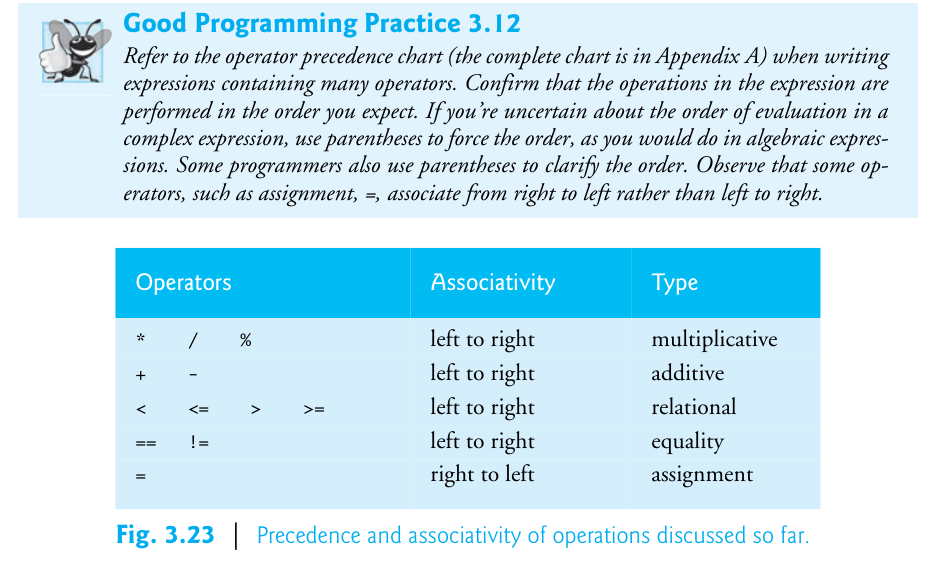
\includegraphics[width=\textwidth]{images/fig3_23_precedence_summary.png}
      {\centering\scriptsize \textbf{Bảng tổng kết độ ưu tiên các toán tử đã học (Hình 3.23)}\par}
    \end{column}

    \begin{column}{0.42\textwidth}
      \begin{block}{\textbf{Thứ tự từ Cao xuống Thấp:}}
        \begin{enumerate}\small
          \item \textbf{Ngoặc đơn:} \texttt{()}
          \item \textbf{Số học nhân chia:} \texttt{*}, \texttt{/}, \texttt{\%}
          \item \textbf{Số học cộng trừ:} \texttt{+}, \texttt{-}
          \item \textbf{Quan hệ:} \texttt{<}, \texttt{<=}, \texttt{>}, \texttt{>=}
          \item \textbf{Bình đẳng:} \texttt{==}, \texttt{!=}
          \item \textbf{Toán tử gán:} \texttt{=} (kết hợp phải)
        \end{enumerate}
      \end{block}
      \begin{exampleblock}{\textbf{Ghi nhớ:}}
        Toán tử số học luôn được tính trước toán tử so sánh, và toán tử gán luôn thực hiện cuối cùng!
      \end{exampleblock}
    \end{column}
  \end{columns}
\end{frame}

% ==============================================================================
% SLIDE 42: CHUẨN MỰC CLEAN CODE MICROSOFT
% ==============================================================================
\begin{frame}{Quy chuẩn Viết Code Sạch (Microsoft C\# Coding Conventions)}
  \begin{columns}[T]
    \begin{column}{0.48\textwidth}
      \begin{block}{\textbf{1. Quy chuẩn Đặt tên (Naming):}}
        \begin{itemize}\small
          \item \textbf{PascalCase:} Dành cho tên Lớp (\texttt{class Welcome1}) và tên Phương thức (\texttt{Main}, \texttt{WriteLine}).
          \item \textbf{camelCase:} Dành cho tên biến cục bộ (\texttt{number1}, \texttt{sum}) và tham số phương thức.
          \item Đặt tên có ý nghĩa gợi nhớ (\textit{meaningful names}): tránh đặt tên cẩu thả như \texttt{a}, \texttt{b}, \texttt{x123}.
        \end{itemize}
      \end{block}
    \end{column}

    \begin{column}{0.48\textwidth}
      \begin{block}{\textbf{2. Khoảng trắng \& Bố cục (Layout):}}
        \begin{itemize}\small
          \item Đặt dấu cách quanh các toán tử nhị phân: \texttt{sum = a + b;} thay vì \texttt{sum=a+b;}.
          \item Đặt dấu cách sau dấu phẩy: \texttt{int a, b, c;}.
          \item Thụt lề chuẩn 3 hoặc 4 khoảng trắng cho mỗi khối lệnh con.
          \item Đặt dấu mở ngoặc \texttt{\{} trên một dòng riêng biệt theo phong cách chuẩn Allman của C\#.
        \end{itemize}
      \end{block}
    \end{column}
  \end{columns}
  \vspace{2mm}
  \begin{alertblock}{\textbf{Tác phong kỹ sư:}}
    Mã nguồn sạch sẽ phản ánh tư duy logic mạch lạc của người kỹ sư, giúp giảm 70\% thời gian gỡ lỗi!
  \end{alertblock}
\end{frame}

% ==============================================================================
% SLIDE 43: HANDS-ON LAB 3: THỰC HÀNH PHÒNG MÁY
% ==============================================================================
\begin{frame}{[HANDS-ON LAB 3] Tự Viết \& Kiểm thử Chương trình \texttt{Comparison}}
  \begin{block}{\textbf{Nhiệm vụ Thực hành Phòng máy (20 Phút):}}
    Sinh viên lớp IT26M tự tay thực hiện các bước sau trên Visual Studio:
    \begin{enumerate}\small
      \item Tạo dự án mới \textbf{Console Application} đặt tên là \texttt{ComparisonApp}.
      \item Đổi tên tệp \texttt{Program.cs} thành \texttt{Comparison.cs}.
      \item Khai báo 2 biến nguyên \texttt{number1} và \texttt{number2}. Nhập dữ liệu từ bàn phím bằng \texttt{Console.ReadLine()} kết hợp \texttt{int.Parse()}.
      \item Viết 6 câu lệnh \texttt{if} độc lập kiểm tra tất cả 6 toán tử: \texttt{==}, \texttt{!=}, \texttt{<}, \texttt{>}, \texttt{<=}, \texttt{>=}.
      \item Sử dụng kỹ thuật \textbf{Nội suy chuỗi C\# 6} (\texttt{\$"..."}) để in kết quả định dạng rõ nét.
    \end{enumerate}
  \end{block}

  \begin{exampleblock}{\textbf{Kiểm thử với các bộ dữ liệu biên (Edge Cases):}}
    \begin{itemize}\small
      \item \textbf{Test 1 (Hai số bằng nhau):} Nhập 50 và 50 $\to$ Kiểm tra xem có xuất đúng 3 dòng (\texttt{==}, \texttt{<=}, \texttt{>=})?
      \item \textbf{Test 2 (Số âm và số dương):} Nhập -15 và 20 $\to$ Kiểm tra các toán tử \texttt{!=}, \texttt{<}, \texttt{<=}.
    \end{itemize}
  \end{exampleblock}
\end{frame}

% ==============================================================================
% SLIDE 44: KHẢO SÁT BÀI TẬP LỚN & ĐỒ ÁN CUỐI CHƯƠNG
% ==============================================================================
\begin{frame}{Khảo sát Bài tập Lớn \& Đồ án Thực hành Cuối Chương 3}
  \begin{columns}[T]
    \begin{column}{0.32\textwidth}
      \begin{block}{\textbf{1. Vẽ Hình Sao (Ex 3.18)}}
        \small Dùng các lệnh \texttt{Console.Write} và ký tự thoát để in hình hộp chữ nhật, hình bầu dục, mũi tên và kim cương bằng dấu hoa thị \texttt{*}.
      \end{block}
      \centering
      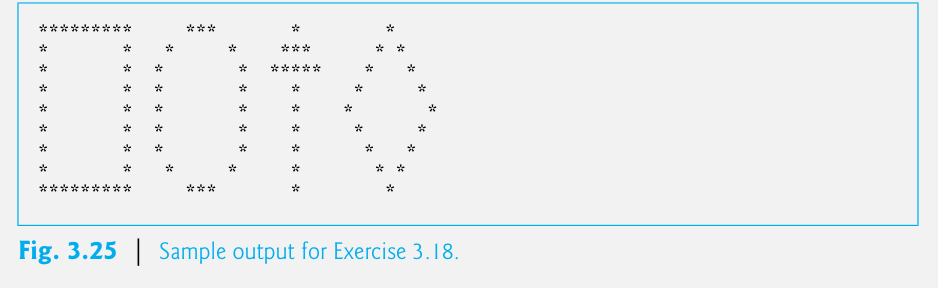
\includegraphics[width=0.9\textwidth]{images/fig3_25_shapes_output.png}
    \end{column}

    \begin{column}{0.32\textwidth}
      \begin{block}{\textbf{2. Bảng Cửu chương (Ex 3.29)}}
        \small Nhập một số nguyên từ bàn phím và in ra bảng nhân 10 dòng bằng các phép toán số học và căn lề ký tự tab \texttt{\textbackslash t}.
      \end{block}
      \centering
      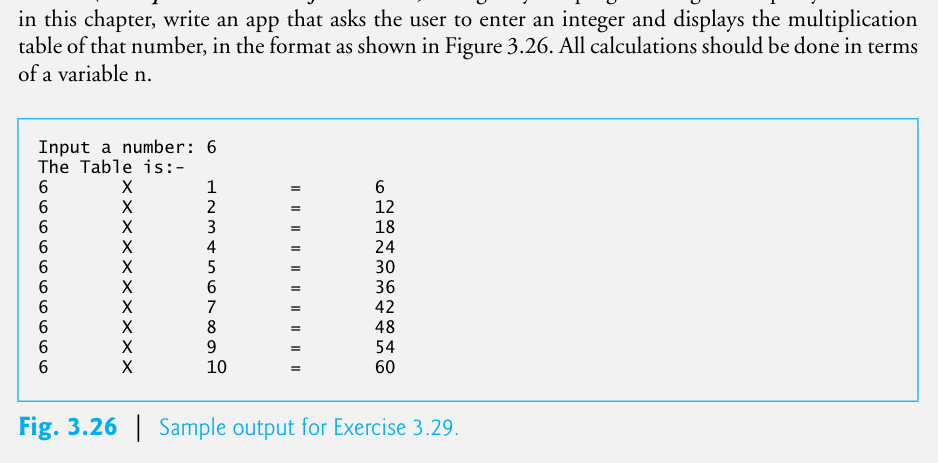
\includegraphics[width=0.9\textwidth]{images/fig3_26_multiplication_table.png}
    \end{column}

    \begin{column}{0.32\textwidth}
      \begin{exampleblock}{\textbf{3. Car-Pool Savings (Ex 3.32)}}
        \small Ứng dụng vì cộng đồng (\textit{Making a Difference}): Nhập quãng đường, giá xăng, tiền đỗ xe $\to$ tính số tiền tiết kiệm hàng ngày khi đi chung xe!
      \end{exampleblock}
    \end{column}
  \end{columns}
\end{frame}

% ==============================================================================
% SLIDE 45: TỔNG KẾT CHUẨN ĐẦU RA & DẶN DÒ
% ==============================================================================
\begin{frame}{Tổng kết 5 Chuẩn đầu ra (CLOs) \& Chuẩn bị Chương 4}
  \begin{columns}[T]
    \begin{column}{0.55\textwidth}
      \begin{block}{\textbf{Bảng Checklist Chuẩn đầu ra Buổi học:}}
        \begin{itemize}\small
          \item[$\checkmark$] \textbf{CLO 3.1:} Hiểu cấu trúc Console App, \texttt{Main()}, \texttt{using}, \texttt{class}.
          \item[$\checkmark$] \textbf{CLO 3.2:} Thành thạo \texttt{WriteLine}, escape sequences \& String interpolation.
          \item[$\checkmark$] \textbf{CLO 3.3:} Làm chủ biến \texttt{int}, \texttt{Parse}, cơ chế ô nhớ RAM.
          \item[$\checkmark$] \textbf{CLO 3.4:} Sử dụng 5 phép toán số học, chia nguyên, chia dư \& thứ tự ưu tiên.
          \item[$\checkmark$] \textbf{CLO 3.5:} Ra quyết định bằng câu lệnh \texttt{if} và các toán tử so sánh.
        \end{itemize}
      \end{block}
    \end{column}

    \begin{column}{0.43\textwidth}
      \begin{exampleblock}{\textbf{Nhiệm vụ Về nhà:}}
        \begin{enumerate}\small
          \item Hoàn thành bài tập Self-Review và Exercises 3.7--3.32 trên Cổng Web học tập.
          \item Làm 40 câu trắc nghiệm chuẩn hóa Chương 3.
          \item Đọc trước \textbf{Chương 4: Introduction to Classes, Objects, Methods and strings}.
        \end{enumerate}
      \end{exampleblock}
      \begin{center}
        \textbf{\large CẢM ƠN CÁC EM SINH VIÊN IT26M!}
      \end{center}
    \end{column}
  \end{columns}
\end{frame}

\end{document}
